\documentclass{scrartcl}
\setkomafont{disposition}{\normalfont\bfseries}
\usepackage[utf8]{inputenc}
\usepackage{natbib}
\usepackage{graphicx}
\usepackage[francais]{babel}
\usepackage[T1]{fontenc}
\usepackage{xcolor}
\usepackage{mathtools}
\usepackage{hyperref}
\usepackage{amsmath}
\usepackage{listings}
\usepackage{calc}
\usepackage{xparse}
\usepackage{framed}
\usepackage[htt]{hyphenat}
\usepackage{amssymb}
\usepackage{amsfonts}
\usepackage{tabularx}
\usepackage{makecell}
\usepackage{float}
\usepackage[toc,page]{appendix}
\usepackage[nottoc]{tocbibind}
\renewcommand\appendixtocname{Annexes}
\renewcommand\appendixpagename{Annexes}

\lstset{ 
  basicstyle=\footnotesize,
  commentstyle=\color{green},
  frame=single,
  keywordstyle=\color{blue},
  language=Java,
  rulecolor=\color{black},
  stringstyle=\color{red},
  tabsize=2,
  title=\lstname,
  moredelim=[il][\textcolor{orange}]{\$\$},
  moredelim=[is][\textcolor{orange}]{\%\%}{\%\%}
}

\newcommand{\project}{$\mathbf{\Pi}$}
\newcommand{\classUniverse}{$\mathbf{U}$}
\newcommand{\category}{$\mathbf{C}$}
\newcommand{\class}{$c$}

\newcommand{\categoryUniverse}{$\mathbf{P}$}
\newcommand{\dependantClasses}{$\mathbf{DaC}$}
\newcommand{\dependedClasses}{$\mathbf{DeC}$}
\newcommand{\numberOfMethod}{$\mathbf{NoM}$}
\newcommand{\numberOfabstractMethod}{$\mathbf{NoAM}$}

% Macro structuration des besoins. Trois arguments (dans l'ordre) :
% - Titre;
% - Priorité (Faible, Moyenne ou Forte);
% - Description;
\newcommand{\requirement}[3] {
    \vbox{
        \begin{framed}
            {\centering \textbf{\underline{#1}}\\[0.25 cm]\par}
            \begin{itemize}
                \item \textbf{Priorité} : #2
                \item \textbf{Description} : #3
            \end{itemize}
        \end{framed}
    }
}

\newcommand{\TODO}[1] {
    \noindent \paragraph{\textcolor{red}{#1}}
}

\title{Mémoire}
\author{Delrée Sylvain, Giachino Nicolas, Martinez Eudes, Ousseny Irfaane}
\date{Jeudi 4 Avril 2019}
\makeatletter
\let\thetitle\@title
\let\theauthor\@author
\let\thedate\@date
\makeatother

\begin{document}

\begin{titlepage}
	\centering
    \vspace*{0.5 cm}
    
\includegraphics[scale = 0.5]{img/logo.jpg}\\[1.0 cm]
    \textsc{\LARGE PdP - Métriques de Maintenabilité}\\[1.0 cm]
	\rule{\linewidth}{0.2 mm} \\[0.4 cm]
	{\huge \bfseries \thetitle}\\
	\rule{\linewidth}{0.2 mm} \\[0.5 cm]
	{\small \thedate}\\[0.5 cm]
	{\small Dépôt Savane :\\ \url{https://services.emi.u-bordeaux.fr/projet/savane/projects/pdp2019mm/}}\\[1.5 cm]
	\begin{minipage}{0.4\textwidth}
		\begin{flushleft} \large
			\emph{Soumis pour :}\\
			(Client) Narbel Philippe\\
            (Chargé de TD) Hofer Ludovic\\
		\end{flushleft}
	\end{minipage}~
	\begin{minipage}{0.4\textwidth}
        \begin{flushright} \large
			\emph{Soumis par :} \\
			Delrée Sylvain\\
            Giachino Nicolas\\
            Martinez Eudes\\
            Ousseny Irfaane\\
		\end{flushright}
	\end{minipage}\\[2 cm]
\end{titlepage}
\tableofcontents
\pagebreak










                    % ------------------------------------- %
                    % -------------> CONTENT <------------- %
                    % ------------------------------------- %

\section{Introduction}
    
    \paragraph{}Lors du développement de systèmes logiciels de taille conséquente, se contenter d'en écrire le code ne suffit pas. En effet, sans exercer une réflexion sur la manière dont il est préférable de séparer et d'organiser les éléments de ceux-ci, il devient rapidement complexe d'en conserver une vue d'ensemble claire. Le processus de maintenance s'en trouve directement impacté. Il devient alors impératif d'élaborer une architecture pour de tels logiciels.


    \paragraph{}Dans ce contexte, étudier en profondeur les éléments qui semblent rendre un design flexible, robuste et maintenable ainsi que fournir des outils qui permettent l'extraction et l'analyse de ces éléments constitue une priorité. En effet, être capable de déterminer le degré de maintenabilité d'un projet permettrait aux développeurs d'effectuer un suivi de la qualité de leur application. Ceci rendrait le développement et la maintenance plus aisés.

    \paragraph{}Dans le cadre de l'unité d'enseignement \og Projet de Programmation\fg, la métrique définie par Martin\cite{Martin:1994} va être au centre de notre projet. Cette dernière permet, au travers d'une analyse des dépendances, une étude de la maintenabilité d'un projet de développement logiciel.

    \paragraph{}Dans le cas de notre projet, l'application que nous devrons mettre en œuvre reçoit en entrée un programme de paradigme Orienté Objet. Elle devra réaliser une analyse au moyen de métriques logicielles afin d'obtenir des informations sur la maintenabilité en sortie.

\begin{figure}[ht]
    \centering
    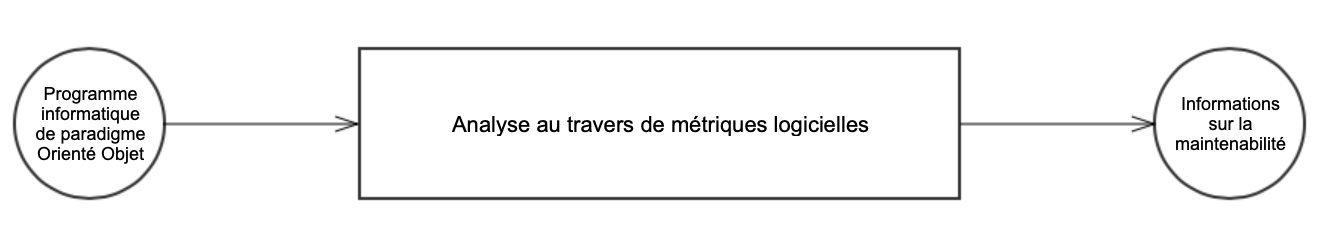
\includegraphics[scale=0.60]{img/intro.png}
    \caption{Vision simplifiée du fonctionnement de l'application} 
    \label{fig:intro}
\end{figure}
    




                    % ------------------------------- %
                    % ----------> DOMAINE <---------- %
                    % ------------------------------- %

\newpage
\section{Description du domaine}

    \begin{abstract}
        Cette section a pour vocation de décrire la métrique utilisée ainsi que tout le vocabulaire nécessaire à sa compréhension.
    \end{abstract}

\subsection{Préambule}

    \paragraph{}Le domaine dans lequel s'inscrit l'application est celui de l'architecture logicielle. En effet, il s'agit ici de déterminer un indicateur du degré de qualité qu'un logiciel possède au regard de la manière dont sont structurés ses composants. Bien que de nombreuses métriques aient été élaborées dans ce but, le programme s'appuiera sur celle définie par Robert Martin\cite{Martin:1994}. Cette étude s'intéressera à son application au paradigme orienté objet. 
    
\subsection{Concepts}
\label{mm:concepts}

\subsubsection{Dépendance et granularité}
    \paragraph{Granularité}La granularité \emph{de structure} (par la suite nous utiliserons simplement le terme de granularité) est une échelle de groupement hiérarchique des éléments constitutifs d'un programme. Chaque niveau de granularité est une partition de l'ensemble de ces éléments. Des exemples de niveaux de granularité dans un programme orienté objet sont :
    \begin{itemize}
        \item Les attributs et méthodes.
        \item Les classes et objets.
        \item Les packages, les namespaces.
        \item Les super-packages.
    \end{itemize}
    Les éléments d'un niveau de granularité sont appelés \textbf{granules}. Chaque granule d'un niveau contient un ensemble de granules du niveau du dessous.
    
    \paragraph{Dépendance}Soient A et B des granules, le plus souvent du même niveau. A \emph{dépend} de B dans le cas où A utilise B dans sa définition. Cette relation de dépendance peut s'exprimer sous différentes formes :
    \begin{itemize}
        \item \textbf{Dépendance par héritage} : A réutilise globalement B.
        \item \textbf{Dépendance par association} : A possède une référence directe vers B.
        \item \textbf{Dépendance par utilisation} : A communique avec B.
    \end{itemize}

    \paragraph{Couplage}Le degré de couplage est une mesure de l'\emph{interdépendance} entre les différents granules d'un même niveau. On parle de couplage fort pour signifier que l'interdépendance est élevée.

    \paragraph{Cohésion}La cohésion représente le degré de liaison, de collaboration et d'interdépendance entre les éléments appartenant à un même granule. Une forte cohésion implique que le granule se concentre sur un seul et unique but, une seule et même responsabilité : réaliser des traitements relatifs uniquement à l’intention de celui-ci.
    
    \paragraph{Principe de simplification min-max}Pour deux niveaux de granularité consécutifs, il faut favoriser une cohésion forte et un couplage faible.

\subsubsection{Propriétés d'un design}

    \paragraph{}Afin de comprendre la métrique détaillée dans ce document, il est nécessaire de définir plusieurs propriétés qu'une architecture logicielle peut posséder (ceux-ci sont repris de l'article fondateur de cette métrique, définie par Robert Martin\cite{Martin:1994}) :

    \paragraph{Rigidité}Un design rigide est un design qui ne peut être facilement changé. C'est souvent le cas si les composants d'un système sont trop interdépendants. Dans ce cas, un changement dans un composant peut forcer beaucoup d'autres composants à changer également et son impact peut être difficile, si ce n'est impossible, à évaluer.

    \paragraph{Fragilité}Un design fragile est un design qui a tendance à cesser de fonctionner à plusieurs endroits si un seul changement est effectué. Dans la plupart des cas, les problèmes engendrés par cette modification surviennent à des endroits sans relation conceptuelle avec la partie ayant subi la modification. De plus, la correction de ces erreurs amène souvent à davantage de nouveaux problèmes.

    \paragraph{Robustesse}Un design robuste est l'exact opposé d'un design fragile. En effet, est considéré comme robuste un design au sein duquel un unique changement ne cause pas toute une cascade de problèmes.

    \paragraph{Maintenabilité}Un design maintenable est un design qui peut facilement évoluer. Il faut comprendre par là qu'il doit être facile d'ajouter de nouvelles fonctionnalités ou de modifier le comportement de celles déjà existantes. Un design rigide ou fragile sera peu maintenable.

    \paragraph{Réutilisabilité}Un design réutilisable est un design qui permet la réutilisation de certains de ses composants sans nécessiter d'embarquer ceux dont on ne veut pas. Si ses composants dépendent fortement les uns des autres, le design est dit difficile à réutiliser car il est compliqué d'isoler les composants désirés.
    
\subsubsection{Propriétés d'un composant}
\label{componentProperties}

    \paragraph{}Il s'agit ici de définir plusieurs propriétés que peuvent avoir les composants d'un logiciel. Ces propriétés interviennent dans le calcul de la métrique détaillée plus bas.
    
    \paragraph{Responsabilité}Un composant responsable est un composant dont dépendent d'autres composants. Un tel composant a intérêt à ne pas être souvent modifié car chaque changement peut se diffuser aux composants dépendant de lui.
    
    \paragraph{Indépendance}Un composant est dit indépendant s'il ne dépend d'aucun autre. Cette notion peut être nuancée : on peut admettre qu'un composant est très indépendant s'il dépend de peu d'autres et peu indépendant s'il dépend de beaucoup d'autres. Un composant très indépendant sera peu amené à changer à cause d'autres composants, de par son faible nombre de dépendances.
    
    \begin{figure}[ht]
        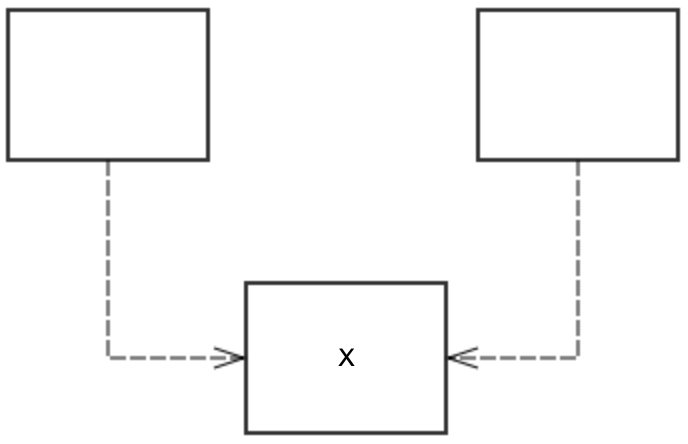
\includegraphics[width=\textwidth/2]{img/StableGranule.png}
        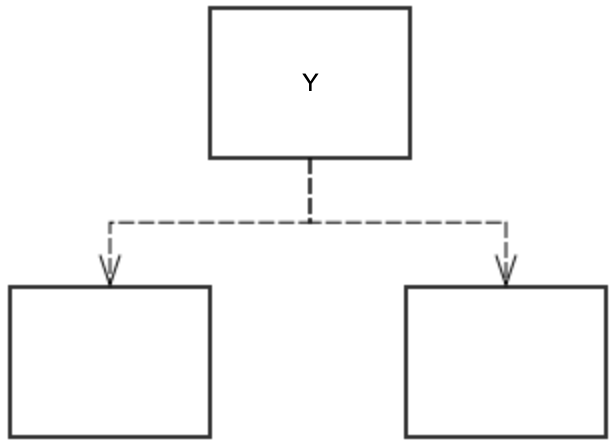
\includegraphics[width=\textwidth/2]{img/InstableGranule.png}
        \caption{Un granule stable X et un granule instable Y}
    \end{figure}
    
    
    \paragraph{Stabilité}La stabilité est une propriété combinant les deux précédentes. En effet, joue en faveur de la stabilité d'un composant :
    \begin{itemize}
    	\item Le nombre de composants dépendant de lui (\emph{responsabilité}).
    	\item L'absence de composants dont il dépend (\emph{indépendance}).
    \end{itemize}
    La combinaison d'une forte responsabilité et d'une importante indépendance est synonyme de forte stabilité et vice versa. La stabilité vise à fournir une indication de la tendance qu'un composant aura à changer dans le temps. Plus le composant est stable, plus cette tendance est faible. En effet, un composant responsable aura peu tendance à changer à cause de la propagation des changements que cela peut engendrer. De même, un composant indépendant aura moins tendance à changer que s'il avait beaucoup de dépendances car une modification extérieure a peu de chances de se répercuter sur lui.
    
    \paragraph{Stable Dependency Principle (SDP)}Selon le SDP énoncé par Martin\cite{Martin:2003}, une bonne dépendance (\emph{Good dependency}) est une dépendance dont la cible est très stable. Si A dépend de B et que B est très stable, alors cette dépendance est très bonne. Par opposition, une mauvaise dépendance (\emph{Bad dependency}) est une dépendance dont la cible est instable. Ce sont, assez naturellement, ces dépendances qu'il faut éviter.
   
    \paragraph{Niveau d'abstraction}L'abstraction, ou le niveau d'abstraction, désigne la proportion d'un composant qui est abstraite (c.à.d. une partie ne comportant que des signatures et pas d'implémentation, dans le but d'être héritée et définie ailleurs). Plus un composant contient de parties abstraites par rapport à sa taille totale, plus il est lui-même abstrait.
    

    \paragraph{Stable Abstraction Principle (SAP)}Le SAP décrit par Martin\cite{Martin:2003} est un principe qui met en relation les concepts de stabilité et d'abstraction. Ce principe stipule :
    \begin{itemize}
        \item qu'un composant stable doit également être abstrait pour que sa stabilité ne l'empêche pas d'être étendu (à comprendre ici dans le sens de fournir des alternatives, sous forme d'\emph{extensions horizontales} proposant plusieurs implémentations distinctes). 
        \item qu'un composant instable doit également être concret, car son instabilité permet de modifier facilement le code concret qu'il contient.
    \end{itemize}

    
\subsection{Métrique de Martin}
\subsubsection{Présentation et définitions}

    \paragraph{}La métrique de Martin a été définie pour la première fois en 1994 par Robert Martin\cite{Martin:1994}. L'auteur l'a par la suite citée au sein d'autres ouvrages\cite{Martin:2003}, et une large bibliographie scientifique mentionne, critique et complète celle-ci\cite{HyryLepp:2009}\cite{BUmetric:2016}\cite{KaurShar:2015}\cite{Spinellis:2006}\cite{Pressman:2000}. La métrique s'articule autour de deux notions centrales : la stabilité et le niveau d'abstraction (cf. \ref{componentProperties}).


    \paragraph{Composantes}Martin présente une métrique principale : la distance entre un \textit{granule} représenté par un point de coordonnées (Instabilité, Abstraction) et la \emph{Main Sequence} (définie plus précisément ci-dessous), une droite représentant le positionnement idéal des granules. Plus cette distance est grande, moins le granule correspond au modèle recherché. Afin de calculer cette distance, il est nécessaire de calculer plusieurs autres métriques, qui s'appliquent toutes à un granule :
    \begin{itemize}
        \item \textbf{Couplage Afférent} (\emph{Afferent Coupling}), noté \textbf{Ca} : Il s'agit du nombre de granules externes qui dépendent du granule.
        \item \textbf{Couplage Efférent} (\emph{Efferent Coupling}), noté \textbf{Ce} : Il s'agit du nombre de granules externes dont dépend le granule.
        \item \textbf{Instabilité} (\emph{Instability}), notée \textbf{I} : Il s'agit d'une quantification de l'instabilité du granule qui fait intervenir les métriques de couplage (Ca et Ce).
        \item \textbf{Niveau d'abstraction} (\emph{Abstractness}), noté \textbf{A} : Il s'agit d'une quantification du niveau d'abstraction du granule.
        \item \textbf{Distance} (Distance par rapport à la Séquence Principale), notée \textbf{D} (ou \textbf{Dn} pour la version normalisée) : Il s'agit d'une mesure de la distance perpendiculaire du granule à la Séquence Principale. Cette distance donne une idée de la qualité du granule : le but est de minimiser cette valeur.
    \end{itemize}

\begin{figure}[ht!]
    \centering
    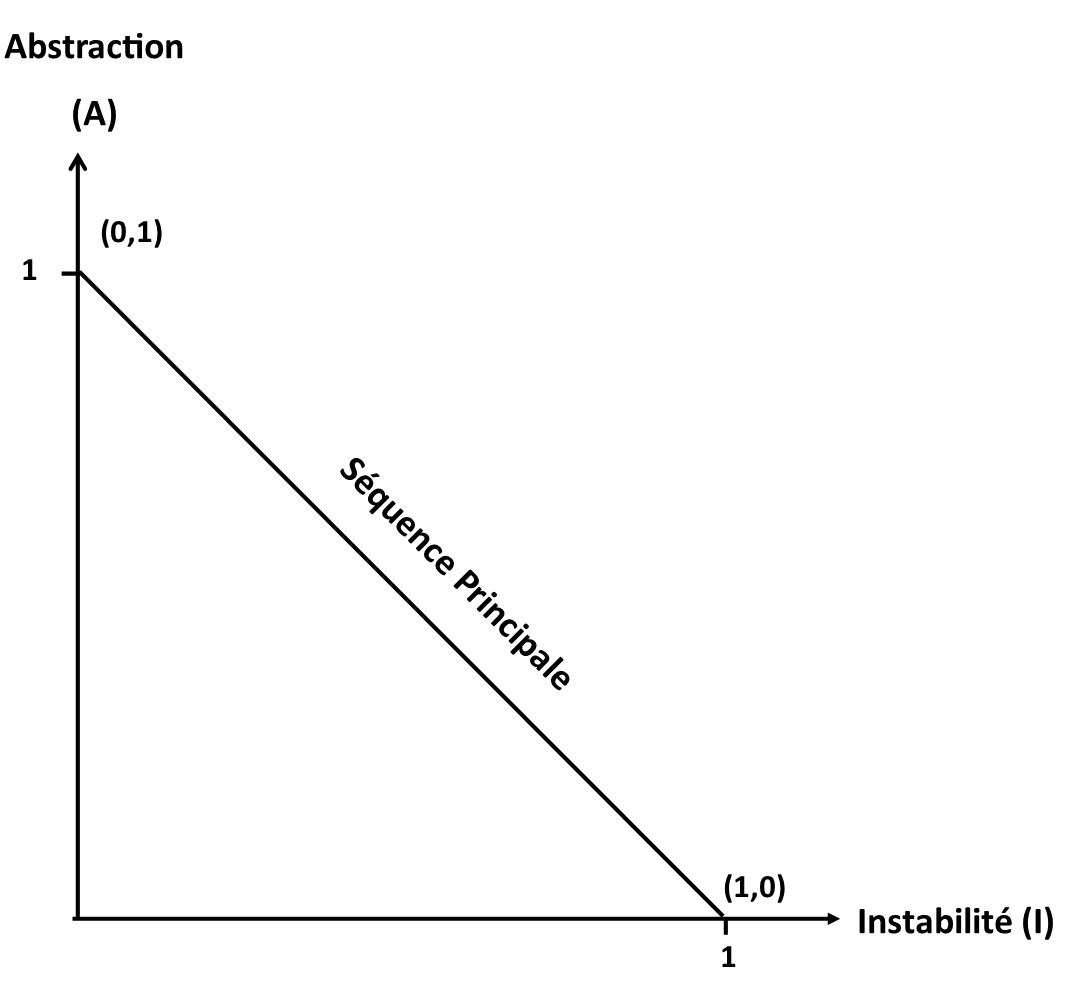
\includegraphics[scale=0.2]{img/MainSequence.png}
    \caption{Séquence principale}
    \label{fig:mainSeq}
\end{figure}

    \paragraph{}Il est également nécessaire de définir ce qu'est la \textbf{Séquence Principale} (\emph{Main Sequence}). Elle intervient dans le contexte d'une représentation en deux dimensions des métriques. Dans ce plan, un granule est représenté par un point dont les coordonnées sont les suivantes : \textbf{(Instabilité, Niveau d'Abstraction)}. Les positions idéales se situent en coordonnées (1,0) : il s'agit d'un granule instable mais entièrement concret ; ainsi qu'en (0,1) : il s'agit d'un granule stable et entièrement abstrait. Des compromis sont également possibles : il s'agit de la Séquence Principale, une droite passant par (1,0) et (0,1). Cette droite est la représentation du SAP. Les granules proches de cette droite sont donc considérés comme bien équilibrés selon ce principe.
    


\subsubsection{Formalisation}
    \label{martin:formalisation}
    \paragraph{Catégorie de classe}La métrique exposée par Martin dans l'article \textit{OO Design Quality Metrics : an Analysis of Dependencies}\cite{Martin:1994} publié en 1994, a pour but d'étudier les dépendances entres les différentes \textbf{catégories de classes} (\emph{class categories}) d'un programme. 
    
    La notion de catégorie de classes est ici empruntée à Grady Booch\cite{Booch:1991}. Une catégorie de classes est définie comme un ensemble de classes interdépendantes et cohésives partageant un but commun.
    
    \paragraph{Granularité package}En 2003, dans son livre\cite{Martin:2003}, R. Martin redéfinit la granularité sur laquelle s'applique la métrique. Le concept de catégorie de classes devient plus concret : il s'intéresse ici au niveau de granularité des packages. Il y expose également différents principes d'organisation des packages tels que le SDP et le SAP qui sont sous-jacents à la métrique. Dans la suite de cette sous-section, on considérera donc un granule comme étant un package.



    \paragraph{Composition de la métrique}La métrique de Martin est constituée des 5 composantes : Ca, Ce, I, A et D, définies précédemment. On appellera \textbf{composantes primordiales} de la métrique les composantes Ca, Ce, et A. Celles-ci doivent être calculées à partir des \textbf{données extractibles}. On appelle données extractibles l'ensemble des données nécessaires à l'application de la métrique de Martin. Les composantes I et D sont déterminées à partir des composantes primordiales.
    
    \paragraph{Notations}On considère :
    \begin{itemize}
        \item \project{}, un projet de programmation.
        \item \granule{} $\in$ \project{} un granule (package) appartenant au projet.
        \item \granuleUniverse{} $\coloneqq \{$\granule{}$ \, | \, $ \granule{} $\in$ \project{}$\}$, l'ensemble ou univers des granules composant le projet.
    \end{itemize}
    Afin d'exprimer les formules de calcul des composantes de la métrique, on utilisera les notations :
    \begin{itemize}
        \item \dependantClasses{}(\granule{}, \granuleUniverse{}) = Le nombre de classes dans l'univers \granuleUniverse{} de \granule{} dépendant de \granule{}.
        \item \dependedClasses{}(\granule{}, \granuleUniverse{}) = Le nombre de classes dont dépend \granule{} dans son univers \granuleUniverse{}.
        \item \numberOfClass{}(\granule{}) = Le nombre de classes présentes au sein de \granule{}.
        \item \numberOfabstractClass{}(\granule{}) = Le nombre de classes abstraites présentes au sein de \granule{}.
    \end{itemize}
    
    \paragraph{Données extractibles}Les données extractibles sont représentées par le tuple $(G, A)$ défini sur \granuleUniverse{} par :
    \begin{itemize}
        \item $G = (V, E)$, le graphe des dépendances où $V = $ \granuleUniverse{} et $E = \{i \to j \, | \, i $ dépend de $j\}$.
        \item $A \coloneqq$ (\granule{}, \numberOfClass{}(\granule{}), \numberOfabstractClass{}(\granule{})) un 3-uplet représentant les données d'abstraction.
    \end{itemize}
    
    \paragraph{Calcul des composantes}Les différents composants de la métrique définis plus haut sont ainsi calculables à l'aide des formules suivantes : 
    \begin{itemize}
        \item Ca(\granule{}) = \dependantClasses{}(\granule{}, \granuleUniverse{}) $\in \mathbb{N}$
        
        \item Ce(\granule{}) = \dependedClasses{}(\granule{}, \granuleUniverse{}) $\in \mathbb{N}$
        
        \item A(\granule{}) = \numberOfabstractClass{}(\granule{}) /
        {\numberOfClass{}(\granule{})} $\in [0, 1]$

        \item I(\granule{}) = Ce(\granule{}) / (Ca(\granule{}) + Ce(\granule{})) $\in [0, 1]$
        
        \item Dn(\granule{}) = |(A(\granule{}) + I(\granule{}) - 1)| $\in [0, 1]$.
    \end{itemize}

    \paragraph{}La multiplicité des dépendances entre deux granules \granule{}$_1$ et \granule{}$_2$ est relative au nombre de dépendances distinctes entre \granule{}$_1$ et \granule{}$_2$. La métrique de Martin considère cette multiplicité dans les calculs effectués. En revanche, Martin ne fait pas allusion à l'importance des dépendances (selon le type).
    



\subsubsection{Critiques et pistes d'amélioration}

    \paragraph{}Les résultats de la métrique de Martin, et des métriques logicielles en général, ne constituent pas une référence absolue. Leur intérêt est de fournir des indicateurs qui peuvent servir à détecter les zones d'un programme auxquelles prêter une attention particulière.
    
    \paragraph{Combinaison d'indicateurs}Dans l'optique de mesurer le degré de maintenabilité d'un logiciel, il est possible d'étudier celui-ci sous le prisme de différentes métriques.
    Par exemple, Chidamber et Kemerer ont défini en 1994 un ensemble de métriques\cite{ChidamberKemerer:1994} qui permettent d'obtenir des indicateurs plus simples à étudier que ceux résultant de la métrique de Martin. Ces métriques portent sur l'étude du couplage et de la cohésion à différents niveaux de granularité.
    Dans cet ensemble, on trouve des métriques telles que : la profondeur de l'arbre d'héritage (métrique \textbf{DIT}), le nombre de fils d'une classe (métrique \textbf{NOC}) et le degré de cohésion des méthodes d'une classe (métrique \textbf{LCOM}).
    
    \begin{quote}
        These metrics should assist software designers in their understanding of the complexity of their design and help direct them to simplifying their work. What the designers should strive for is strong cohesion and loose coupling.
        \begin{flushright}--- C. Kemerer \& S. Chidamber \cite{ChidamberKemerer:1994} (p.229)\end{flushright}
    \end{quote}

    \paragraph{Granularités}Comme explicité dans la section \ref{martin:formalisation}, Martin définit sa métrique comme s'appliquant à la granularité des packages. Cependant, les principes de stabilité et d'abstraction et leur mise en relation peuvent être étudiés à un niveau de granularité inférieur (classes et objets) ou supérieur (super-packages).
    
    \paragraph{Mesure du niveau d'abstraction}La composante A (Abstractness) de la métrique de Martin est calculée à l'aide de la formule : 
    \numberOfabstractClass{}(\granule{}) / {\numberOfClass{}(\granule{})} (c.à.d. le rapport entre le nombre de classes abstraites et le nombre total de classes présentes dans un package). Cette mesure peut-être raffinée afin d'être appliquée au niveau de granularité inférieur. En effet, soit \granule{} un granule représentant une classe. On considère :
    \begin{itemize}
        \item \numberOfMethod{}(\granule{}{}) = Le nombre de méthodes présentes au sein de \granule{}.
        \item \numberOfabstractMethod{}(\granule{}) = Le nombre de méthodes abstraites présentes au sein de \granule{}.
    \end{itemize}
    On peut alors définir le calcul de la composante A comme suit :\\
    {\centering
        A(\granule{}) = \numberOfabstractMethod{}(\granule{}) / \numberOfMethod{}(\granule{}{})
    \par}
    
    \paragraph{Formalisme résultant}Si l'analyse porte sur plusieurs niveaux de granularité, les données extractibles peuvent être récupérées sur le niveau de granularité étudié le plus bas. Les données nécessaires au calcul des métriques sur les niveaux supérieurs pourront être déterminées à partir des données du niveau inférieur.
    
    \paragraph{Multiplicité}Comme explicité dans la partie Formalisation, Martin considère la multiplicité associée à une dépendance d'un granule vers un autre. Certains auteurs (tel que Spinellis\cite{Spinellis:2006}) font l'impasse sur cette donnée dans leurs applications de la métrique de Martin, considérant ainsi qu'une dépendance d'un granule vers un autre est équivalente quelle que soit son importance ou sa multiplicité.

    \paragraph{Pondération}Telle qu'elle est énoncée, la métrique de Martin considère les dépendances comme toutes égales. Or, une dépendance envers un granule stable ne devrait pas avoir le même poids qu'une dépendance envers un granule instable. Afin de raffiner le calcul des métriques, une analyse de la globalité du graphe des dépendances permettrait d'éliminer les dépendances stables du calcul d'instabilité (ou du moins de minimiser leur poids), en considérant qu'une dépendance stable ne rend pas le composant dépendant beaucoup plus instable. Il s'agit d'une exploitation du SDP qui, bien qu'énoncé par Martin, n'influe pas sur le calcul des métriques.
    
    Il serait également possible d'appliquer une pondération relative à l'importance de la dépendance en fonction de son type. On a par ordre d'importance croissant : Dépendance par utilisation, Dépendance par association, Dépendance par héritage.
    
    \paragraph{SAP et Main Sequence}La définition de la Main Sequence (et donc du SAP) donnée par Martin est discutable sur plusieurs points :
    \begin{itemize}
        \item La position idéale en I = 0 et A = 1 est justifiée par le fait qu'un granule stable doive être abstrait pour pouvoir être étendu. Or, un granule concret peut également être étendu et il est même possible de réimplémenter la totalité de son comportement. L'extension d'un granule stable est donc toujours possible, quelle que soit son abstraction.
        \item La position indésirable en I = 1 et A = 1 est justifiée par le fait qu'il n'y ait aucun intérêt à avoir un granule abstrait sans aucun dépendant. Cependant, certaines situations peuvent nécessiter un tel cas de figure. Par exemple, une API peut définir des interfaces qui ont vocation à être implémentées par les clients. Si l'API n'offre aucune implémentation de ces interfaces et les utilise assez peu, une analyse de celle-ci déterminerait que l'instabilité de telles interfaces est proche de 1, bien qu'il s'agisse d'un cas acceptable.
    \end{itemize}


\subsection{Application au langage Java}

    \paragraph{}Notre application a pour objectif d'effectuer les analyses nécessaires au calcul de la métrique de Martin sur des programmes écrits en langage Java. Pour faciliter ce travail, notre application sera elle-même développée en Java (version 8).

\subsubsection{Granularité : Adaptation}
    
    \paragraph{}Chaque langage de programmation propose ses propres structures de modularité. Ceci étant, il est nécessaire de préciser les structures auxquelles s'applique le concept de granularité en fonction du langage dans lequel est écrit le programme que l'on souhaite analyser.
    
    \paragraph{Granules}Les niveaux de granularité principaux qu'on retrouve en Java sont :
    \begin{itemize}
        \item les méthodes et attributs.
        \item les classes.
        \item les packages.
        \item les modules (Java, version 9 ou supérieure).
    \end{itemize}
    Un granule pourra donc désigner n'importe quel élément d'un de ces niveaux. Notre application ne s'intéressera cependant qu'aux niveaux "classes" et "packages".

\subsubsection{Analyse de l'existant}
\label{existingAnalysis}
    \paragraph{}Il existe différents projets qui abordent la question de la maintenabilité de logiciels au travers de l'étude de métriques (on notera que beaucoup d'entre eux exploitent les métriques de Chidamber et Kemerer\cite{ChidamberKemerer:1994}). Certains de ces outils s'intègrent à des IDE comme Eclipse ou IntelliJ, ce qui facilite grandement leur installation et leur utilisation.
    

    \paragraph{JHawk}JHawk\footnote{\url{http://www.virtualmachinery.com/jhawkprod.htm}} est un logiciel propriétaire d'analyse de code source Java. Il est en mesure de calculer un très grand nombre de métriques dont celle de Martin. Il peut être utilisé seul ou en tant que plugin Eclipse.
    
    Il génère plusieurs métriques au niveau des méthodes, classes et packages. En ce qui concerne celle de Martin, il permet d'obtenir :
    \begin{itemize}
        \item Ca et Ce au niveau des classes.
        \item Ca, Ce, A, I et D au niveau des packages.
    \end{itemize}
    A cause du caractère propriétaire de JHawk, il est compliqué de déterminer comment il entreprend ses calculs.
    
    \paragraph{JDepend}JDepend est un logiciel open source dont le code est disponible sur la plateforme Github\footnote{\url{https://github.com/clarkware/jdepend}}. Il met en oeuvre la métrique de Martin (et nourrit donc des ambitions similaires à celles de notre application).

    \paragraph{}JDepend procède à une analyse statique des différents fichiers constituant un projet Java. Plus exactement, il analyse les fichiers compilés (\texttt{.class}) composés de bytecode (il peut également analyser les archives jar).
    
    \paragraph{}A la suite d'une étude du fonctionnement de JDepend, il ressort que celui-ci n'extrait que les informations de dépendance entre les packages. Il extrait les dépendances et calcule ensuite les valeurs de métriques à cette échelle. Il ne peut donc fournir aucune information sur les dépendances entre classes. 
    
    \paragraph{}L'approche du projet décrit dans ce document est différente. En effet, là où JDepend se limite aux packages, notre application adopte une stratégie \textit{bottom-up} : l'analyse s'effectue au niveau des classes (on ne considère pas la granularité des méthodes).
    A partir des résultats de celle-ci, on peut alors calculer les dépendances et métriques des échelles supérieures sans analyse supplémentaire.
    
    \paragraph{}Certains logiciels se basent sur les résultats fournis par JDepend pour analyser des programmes, comme par exemple \textit{Gephi}\footnote{\url{https://dzone.com/articles/visualizing-and-analysing-java}}.






                    % ------------------------------- %
                    % ----------> BESOINS <---------- %
                    % ------------------------------- %

\newpage
\section{Expression des besoins}

    \begin{abstract}
        Dans cette partie, nous allons évoquer l'ensemble des besoins que notre application doit satisfaire.
    \end{abstract}

\subsection{Besoins fonctionnels}

    \requirement{Évaluer les méthodes d'analyse et définir celle à utiliser}
    {Forte}
    {En amont du développement de l'application, les méthodes d'extraction d'informations concernant les dépendances doivent être évaluées. Cela permettra de déterminer si elles offrent les mêmes possibilités ainsi que la facilité à les mettre en place. Une comparaison est disponible en sous-section \ref{methodsComparison}.}

    \requirement{Générer un ensemble de projets annotés (Création d'une vérité terrain)}
    {Forte}
    {Afin de tester notre implémentation, il sera nécessaire de générer une série de projets Java et de fournir les métriques calculées manuellement.

    Dans ces différents cas d'exemple, seule la structure des dépendances (c.à.d. l'agencement des classes, les attributs ainsi que les dépendances liées aux méthodes) est importante. Il sera donc inutile d'implémenter des fonctionnalités spécifiques.}


\subsubsection{Sélection et structuration de l'entrée}

    \requirement{Sélectionner un projet depuis un répertoire local}
    {Forte}
    {L'utilisateur doit pouvoir renseigner un projet en entrée de l'application depuis le système de fichiers de la machine, sous forme de chemin d'accès au répertoire racine de celui-ci.}

    \requirement{Lister récursivement le contenu d'un répertoire}
    {Forte}
    {Pour un répertoire donné, l'application doit être en mesure de lister son contenu. Dans le cas d'une analyse du code source (respectivement, d'une analyse du bytecode), l'application devra pouvoir lister l'arborescence des différents fichiers \texttt{.java} (respectivement \texttt{.class}). Si le répertoire donné ne mène pas à la racine d'un projet Java (sous la forme d'un ensemble de \texttt{.class} ou de \texttt{.java}), l'application devra renvoyer une erreur.}

    \requirement{Créer une structure représentative de l'organisation du projet}
    {Forte}
    {L'application devra créer une structure arborescente contenant tous les packages du projet analysé ainsi que les classes qui les composent.}


\subsubsection{Analyse de fichiers}

    \paragraph{}L'application doit être en mesure de réaliser une \textbf{analyse statique} de fichiers. L'analyse de fichiers consistera en la mesure du niveau d'abstraction des classes ainsi que l'extraction des dépendances. Lors de l'analyse, nous ne nous intéresserons qu'à l'ensemble des dépendances sortantes ; nous pourrons déterminer les dépendances entrantes à partir des premières. Ces mesures permettront de déterminer les composantes Ce et A.

    \requirement{Extraire les dépendances par héritage/implémentation}
    {Forte}
    {L'application devra extraire les dépendances de type héritage/implémentation. Cette information se trouve dans la déclaration de la classe.}

    \requirement{Extraire les dépendances par association}
    {Forte}
    {L'application devra extraire les dépendances de type agrégation/composition. Cette information se trouve dans la liste des attributs de la classe. Cela implique que l'application devra être en mesure de lister les attributs d'une classe et leurs types.}

    \requirement{Extraire les dépendances d'utilisation}
    {Moyenne}
    {L'application devra extraire les dépendances de lien d'utilisation. Il s'agit des variables locales, des appels de méthodes statiques, des paramètres ou des valeurs de retour d'une méthode.}

    \requirement{Extraire les dépendances liées à la généricité}
    {Faible}
    {L'application devra extraire les dépendances dues à la généricité. Cette information peut se trouver dans la déclaration de la classe, dans la signature, dans les attributs ou dans les méthodes. Cette dépendance est plus compliquée à analyser car elle peut prendre plusieurs formes.}
    
    \requirement{Mesurer le nombre de méthodes d'une classe}
    {Forte}
    {Afin d'implémenter la fonction \numberOfMethod{}, il faudra mettre en place une méthode permettant de compter le nombre de méthodes définies par une classe.}
    
    \requirement{Mesurer le nombre de méthodes abstraites d'une classe}
    {Forte}
    {Afin d'implémenter la fonction \numberOfabstractMethod{}, il faudra mettre en place une méthode permettant de compter le nombre de méthodes abstraites définies par une classe.}


\subsubsection{Exploitation de la métrique}

    \requirement{Calculer le couplage afférent (Ca)}
    {Forte}
    {A partir du couplage efférent (Ce) de toutes les classes, l'application devra déterminer le couplage afférent (Ca) de chaque classe en examinant le nombre de classes ayant des dépendances sortantes vers celle-ci.}

    \requirement{Calculer la composante d'instabilité de la métrique}
    {Forte}
    {L'application devra être en mesure d'effectuer le calcul de la composante I de la métrique pour une classe donnée à partir de la formule définie par Martin : I(\granule{}) = Ce(\granule{}) / (Ca(\granule{}) + Ce(\granule{})).}
    

    \requirement{Calculer la composante de distance de la métrique}
    {Forte}
    {L'application devra être en mesure d'effectuer le calcul de la composante Dn de la métrique pour une classe donnée à partir de la formule définie par Martin : Dn(\granule{}) = |(A(\granule{}) + I(\granule{}) - 1)|.}    

    \requirement{Générer un graphe de dépendances}
    {Forte}
    {A partir des dépendances extraites par l'analyse de fichiers, l'application devra pouvoir générer une structure de données représentant l'interdépendance entre les différentes classes du projet : un graphe de dépendances. 
    
    Le graphe de dépendances est défini comme un graphe orienté composé d'un ensemble de $n$ noeuds représentant les $n$ classes de l'analyse et d'un ensemble de $p$ arcs représentant les dépendances entre celles-ci. Étant donné que l'application fait la différence entre chaque type de dépendance, il peut y avoir plusieurs arcs d'un noeud vers un autre (un par type de dépendance).}
    
    \requirement{Calcul des métriques par granularité}
    {Forte}
    {A partir du graphe de dépendances des classes, l'application devra pouvoir passer à un niveau d'échelle supérieur en fusionnant les noeuds pour les regrouper par granule de niveau supérieur (package) et en ne conservant que les arcs sortants et entrants dans ces super-noeuds.}

    \requirement{Générer des tableaux exposant les composantes de la métrique}
    {Forte}
    {L'application devra être en mesure de créer des tableaux exposant les différentes composantes de la métrique : celles récupérées au travers de l'analyse de fichiers (Ce et A) et celles calculées par la suite (Ca, I et D). On pourra obtenir les informations relatives au changement d'échelle à partir des données du graphe de dépendances.}


\subsubsection{Réalisation de rapport d'analyse}

    \paragraph{}L'application devra permettre de générer des fichiers exposant les différentes métriques qu'elle aura traité. Ces fichiers pourront ensuite être interprétés par des outils externes.

    \requirement{Générer des fichiers DOT exposant le graphe des dépendances}
    {Forte}
    {L'application devra être en mesure de générer des fichiers au format DOT. Ces fichiers contiendront les graphes de dépendances calculés précédemment. Il y aura un fichier par échelle d'analyse. Les noeuds contiendront le nom des granules (nom de classe, de package,...), éventuellement associé à leur valeur d'instabilité. Ces fichiers pourront ensuite être interprétés par des outils tels que GraphViz.}
    
    \requirement{Générer des fichiers CSV exposant les métriques}
    {Forte}
    {L'application devra être en mesure de générer des fichiers au format CSV. Ils contiendront les valeurs des différentes composantes de la métrique. Tout comme les fichiers DOT, il en existera un par échelle d'analyse. Ces fichiers pourront ensuite être interprétés par des outils tels que Libre Office Calc.}

    \requirement{Générer une sortie matricielle du graphe}
    {Faible}
    {L'application devra être en mesure de générer des fichiers au format CSV exposant une représentation du graphe sous forme de matrice d'adjacence.}

\subsection{Besoins non fonctionnels}

    \requirement{Documentation}
    {Forte}
    {La documentation de l'application sera scindée en deux documents : l'architecture générale et le manuel d'utilisation. Ceux-ci seront produits dans le format \LaTeX{} afin de permettre leur intégration dans le rapport terminal de l'unité d'enseignement.
    
    \textbf{Architecture générale} : Pour aider les développeurs à modifier / adapter / ajouter des fonctionnalités à l'application.
    
    \textbf{Manuel d'utilisation} : Pour aider l'utilisateur à prendre en main l'application.}

    \requirement{Modularité}
    {Forte}
    {Les algorithmes de calcul des métriques doivent pouvoir être aisément modifiés. L'application doit adopter une architecture lui permettant de s'adapter sans nécessiter de changements conséquents.}

    \requirement{Configuration}
    {Faible}
    {La possibilité de modifier certains paramètres de l'application à l'aide d'un fichier de configuration peut être implémentée en guise d'alternative à la modification directe d'un composant dans le code. Par exemple, il pourrait être possible de paramétrer une pondération à appliquer à chaque type de dépendance dans le calcul de la métrique. La présence d'une telle fonctionnalité est optionnelle.}





\newpage
\section{Architecture}
    \begin{abstract}
        Dans une première sous-partie, nous allons vous présenter le pipeline de notre projet, qui correspond à la chaîne de traitement de notre application. Nous rentrerons ensuite plus en détail dans chaque package en présentant les différentes classes décrivant notre architecture. Finalement, nous traiterons des spécificités techniques qui ont motivé nos choix d'implémentation.
    \end{abstract}
    
\subsection{Pipeline de traitement}

\begin{figure}[ht]
    \centering
    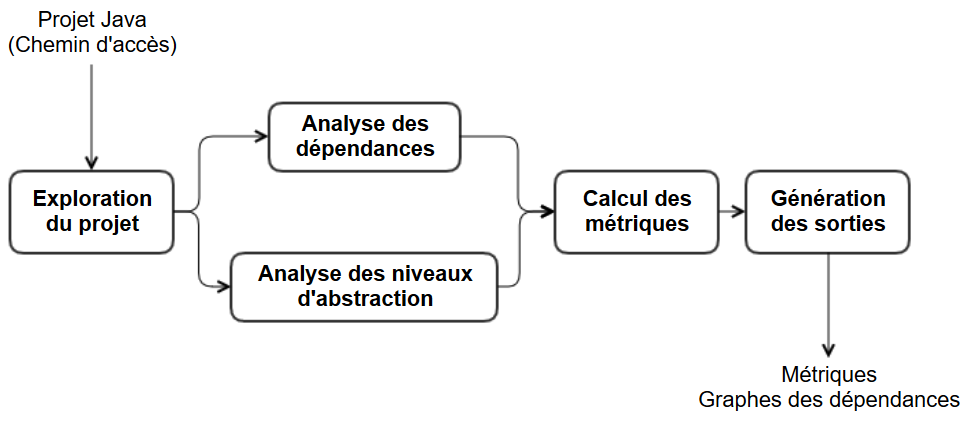
\includegraphics[width=\textwidth]{img/SimplifiedPipeline.png}    
    \caption{Pipeline de traitement de JMetrics}
    \label{fig:simplepipe}
\end{figure}

    \paragraph{}Afin que l'application atteigne son objectif d'obtention de métriques, il est nécessaire de passer par plusieurs étapes afin d'obtenir les informations nécessaires à leur calcul. On peut représenter ces différentes actions sous la forme d'un pipeline de traitement. En effet :

\begin{itemize}
	\item Chaque étape nécessite le résultat de la précédente.
	\item Aucun retour en arrière n'a lieu : une fois une action effectuée, il n'est plus nécessaire d'y revenir plus loin dans l'exécution.
\end{itemize}

    \paragraph{}La figure \ref{fig:simplepipe} illustre le pipeline dans les grandes lignes (il s'agit d'une version plus détaillée de la figure \ref{fig:intro} présente dans l'introduction). L'application est architecturée de manière à ce que chaque package ait la responsabilité de l'exécution d'une étape, chacune ne nécessitant qu'une interaction très limitée avec les autres. Ce pipeline se décompose en quatre phases principales :

    \begin{itemize}
        \bigbreak 
        \item[] \textbf{Exploration du projet (Package \texttt{project})} Dans un premier temps, l'application a besoin de construire une représentation exploitable du projet à analyser. Pour ce faire, celle-ci visite récursivement les répertoires et fichiers composant ce projet et crée une structure arborescente le représentant. La structure ainsi obtenue est ensuite nettoyée afin d'écarter les dossiers vides ou n'ayant que peu d'intérêt (par exemple un dossier n'en contenant qu'un autre).

        \bigbreak 
        \item[] \textbf{Analyse statique des classes (Package \texttt{analysis})} A partir des structures de données précédemment générées, le programme parcourt toutes les classes référencées dans le projet et effectue une analyse de leur code (source ou compilé, en fonction du type d'analyse choisi) afin d'en extraire les données nécessaires au calcul des métriques. Cette étape peut se scinder en deux sous-parties indépendantes et ayant la possibilité d'être effectuées en parallèle :
    	\begin{itemize}
    		\item \textit{Analyse du niveau d'abstraction} : Il s'agit d'effectuer un comptage des méthodes composant la classe et d'en tirer deux valeurs : le \emph{nombre total de méthodes} et le \emph{nombre de méthodes abstraites} de la classe.
    		\item \textit{Analyse des dépendances} : Cette seconde partie est la plus délicate des deux : il s'agit d'extraire les dépendances de la classe vis-à-vis des autres classes du projet. Cette analyse génère une \emph{liste de ces dépendances}.
    	\end{itemize}
	    A partir du résultat de l'analyse des dépendances, l'application génère un graphe pour représenter celles-ci.
	
	    \bigbreak 
	    \item[] \textbf{Calcul des métriques (Package \texttt{metrics})} En utilisant les données renvoyées par l'étape d'analyse, l'application calcule différentes métriques (pour le moment : les métriques de Martin, mais avec possibilité d'extension) pour chaque classe. Les classes sont ensuite regroupées en packages et les valeurs des métriques pour chacun d'eux sont calculées à partir des résultats précédents. Bien que ce ne soit pas le cas pour le moment, une approche similaire pourrait être envisagée pour d'autres niveaux de granularité.
	
	    \bigbreak 
	    \item[] \textbf{Présentation des résultats (Package \texttt{presentation})} Pour finir, les valeurs calculées précédemment doivent être présentées à l'utilisateur. Dans ce but, l'application génère plusieurs fichiers contenant les informations nécessaires (graphe de dépendances au format DOT, tableau de métriques au format CSV, ...).
	\end{itemize}

    \paragraph{}Afin de faciliter la visualisation des données générées par l'application, nous avons mis en place plusieurs scripts \textit{Python}. Ils ne sont cependant que des aides, ne font pas partie du cœur de l'application et ne sont donc pas considérés comme une étape à part entière du pipeline. En outre, un cinquième package (\texttt{graph}) fait partie du projet mais n'a vocation qu'à fournir une structure de graphe partagée entre les autres packages. Il ne constitue donc pas une étape de traitement non plus.

\subsection{Organisation des composants}

\subsubsection{Package project}
    \begin{figure}[h!]
        \centering
        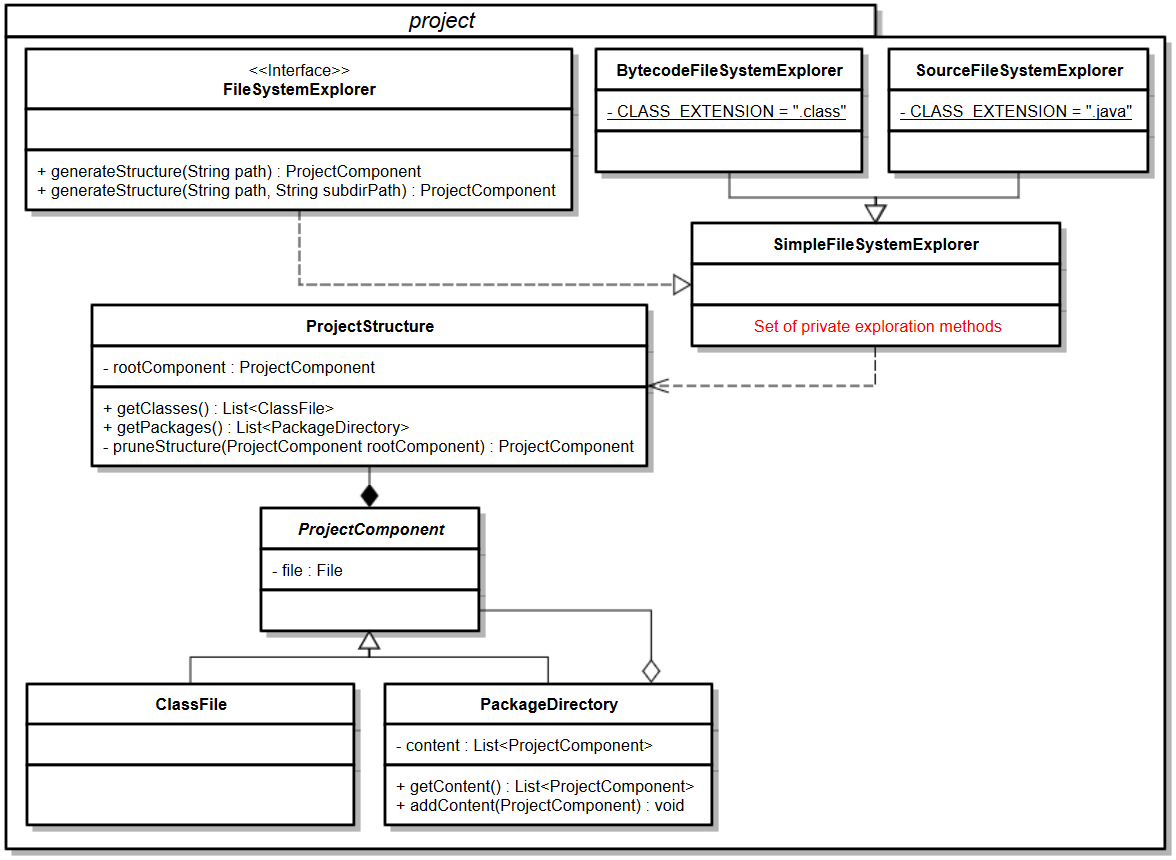
\includegraphics[width=\textwidth]{img/uml/project.png}
        \caption{Diagramme de classes (UML) du package \texttt{project}}
    \end{figure}
	\paragraph{}Le package \texttt{project} fournit les classes nécessaires à l'exploration d'un répertoire donné et à la création d'une représentation de projet Java.

	\paragraph{}Le package est composé des trois éléments suivants :
	\begin{itemize}
		\item Une instance du pattern Composite permet de représenter l’arborescence des composants du projet. Une classe mère \texttt{ProjectComponent} maintient une référence vers un objet \texttt{File}. Les packages sont représentés par la classe composite \texttt{PackageDirectory} exposant un ensemble de \texttt{ProjectComponent}. Les classes sont représentées par la classe feuille \texttt{ClassFile}.
		\item La \texttt{ProjectStructure} est une classe Singleton qui conserve en mémoire la structure du projet qui s’apprête à être analysé et qui fournit des méthodes permettant l’accès aux différents composants de celui-ci (classes et packages). Elle est donc un \emph{repository}.
		\item Enfin, le \texttt{FileSystemExplorer} est un service qui a pour objectif de construire la représentation du projet en explorant le système de fichiers et d’affecter la racine de celle-ci dans la classe \texttt{ProjectStructure}. Notre implémentation du FileSystemExplorer est composée de quatre classes :
		\begin{itemize}
		    \item Une interface \texttt{FileSystemExplorer} qui définit les méthodes d'exploration.
		    \item Une classe abstraite \texttt{SimpleFileSystemExplorer} qui constitue le coeur du processus d'exploration. Elle contient toutes les méthodes nécessaires à cette tâche, permettant une factorisation importante. Le code qu'elle contient est capable de lister tous les fichiers possédant une certaine extension (à définir dans les classes filles).
		    \item Enfin, deux classes concrètes \texttt{BytecodeFileSystemExplorer} et \texttt{SourceFileSystemExplorer} définissent toutes deux les extensions des fichiers à explorer (\emph{.class} et \emph{.java}).
		\end{itemize}
	\end{itemize}
    La structure du projet est construite et parcourue à l'aide d’algorithmes récursifs.
    
\subsubsection{Package analysis}

    \begin{figure}[ht!]
        \centering
        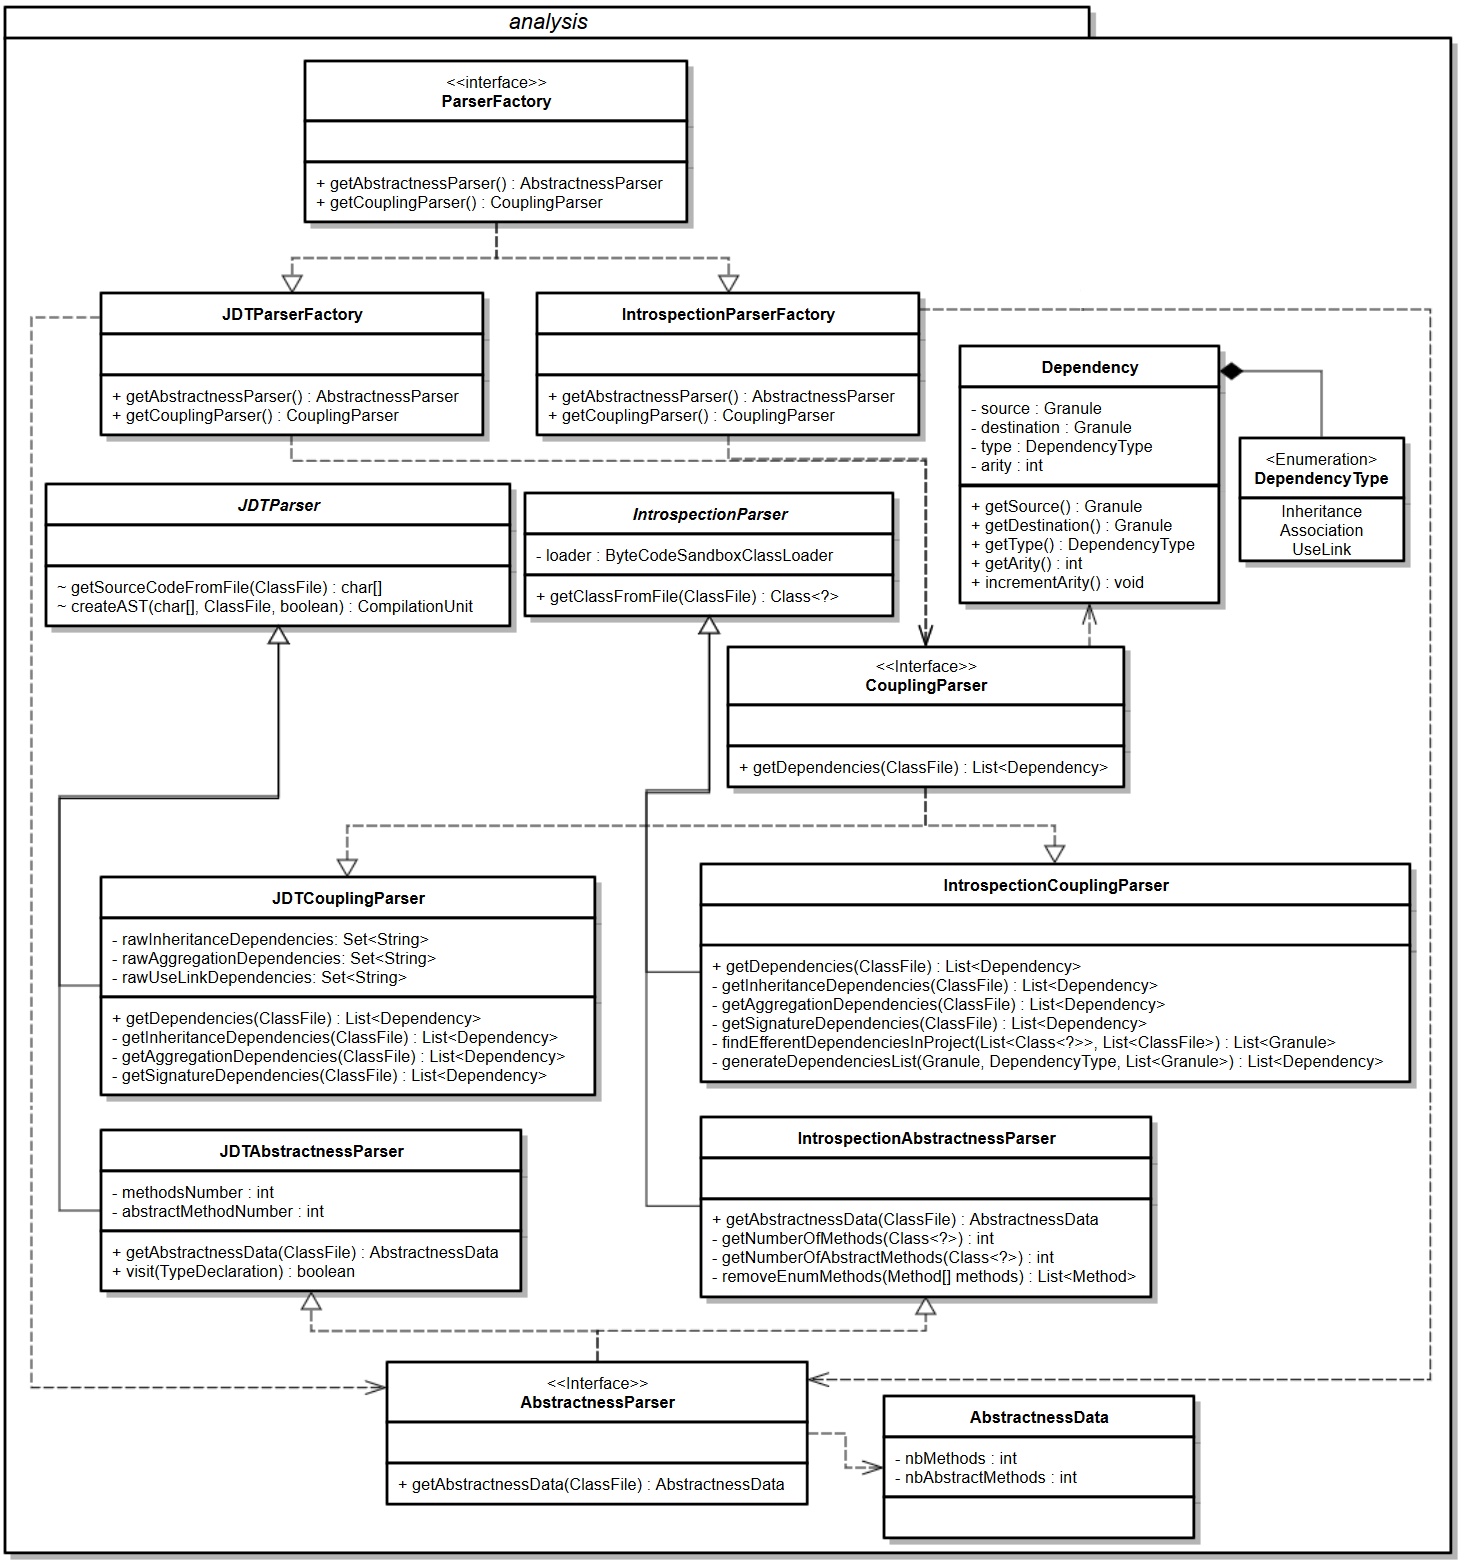
\includegraphics[width=\textwidth]{img/uml/analysis.png}
        \caption{Diagramme de classes (UML) du package \texttt{analysis}}
    \end{figure}

    \paragraph{}Le package \texttt{analysis} contient les composants chargés d'effectuer l'analyse statique du code des classes. Cette analyse est menée à bien par des parseurs. Il en existe deux catégories, chacune définie par une interface :
    \begin{itemize}
    	\item \textbf{AbstractnessParser}, parseur d'abstraction. Il s'agit de l'interface que doivent implémenter tous les parseurs ayant vocation à extraire les informations sur le niveau d'abstraction d'une classe (nombre de méthodes et nombre de méthodes abstraites).
    	\item \textbf{CouplingParser}, parseur de dépendances. Il s'agit de l'interface que doivent implémenter tous les parseurs qui récupèrent les dépendances d'une classe envers les autres.
    \end{itemize}
    Le parseur d'abstraction retourne un objet de la classe \texttt{AbstractnessData}. Cette classe ne possède que deux attributs (\texttt{numberOfMethods} et \texttt{numberOfAbstractMethods}) et les \textit{getters} permettant d'y accéder. Son but est uniquement d'encapsuler ces éléments.
    Le parseur de dépendances, quant à lui, retourne une liste d'objets de la classe \texttt{Dependency}. Cette classe a également pour but d'encapsuler les informations relatives à une dépendance (\texttt{source}, \texttt{destination} et \texttt{type}). Il s'agit d'une représentation intermédiaire avant la construction du graphe de dépendances.
    Dans son état actuel, l'application contient deux implémentations de chacune de ces interfaces : une permettant l'analyse du code source via \emph{l'API Eclipse JDT}\footnote{\url{https://help.eclipse.org/neon/index.jsp?topic=\%2Forg.eclipse.jdt.doc.isv\%2Freference\%2Fapi\%2Foverview-summary.html}} et l'autre servant à l'analyse du code compilé via \emph{l'API d'introspection} \texttt{java.lang.reflect}\footnote{\url{https://docs.oracle.com/javase/8/docs/api/java/lang/reflect/package-summary.html}}. Chaque implémentation est constituée de trois classes :
    \begin{itemize}
    	\item Une implémentation d'\texttt{AbstractnessParser}. Il s'agit de \texttt{IntrospectionAbstractnessParser} et de \texttt{JDTAbstractnessParser}.
    	\item Une implémentation de \texttt{CouplingParser}. Il s'agit de \texttt{IntrospectionCouplingParser} et de \texttt{JDTCouplingParser}.
    	\item Une classe abstraite pour factoriser le code partagé. Il s'agit de \texttt{IntrospectionParser} et de \texttt{JDTParser}.
	\end{itemize}
	L'implémentation utilisant le JDT a une particularité supplémentaire. En effet, l'API JDT faisant usage du pattern \emph{Visitor} pour parcourir le code source, les deux parseurs implémentent ce pattern. Il existe donc une méthode \emph{visit} pour chaque élément du code source (déclaration de classe, de méthode, ...) permettant de récupérer les informations recherchées.
	
	\paragraph{}Afin de faciliter l'instanciation des parseurs par le code client, une interface \texttt{ParserFactory} est définie et implémentée pour fournir une \emph{factory} pour chacune des deux familles de parseurs (introspection et JDT) : \texttt{IntrospectionParserFactory} et \texttt{JDTParserFactory}. Pour le code client, il est obligatoire de passer par une de ces \emph{factory} car les constructeurs des parseurs ne sont accessibles que dans leur propre package.
	
	\paragraph{}Enfin, ce package définit également les différents types de dépendances (\emph{Inheritance}, \emph{Association} et \emph{UseLink}) au sein de l'énumération \texttt{DependencyType}.
    
\subsubsection{Package graph}

    \begin{figure}[H]
        \centering
        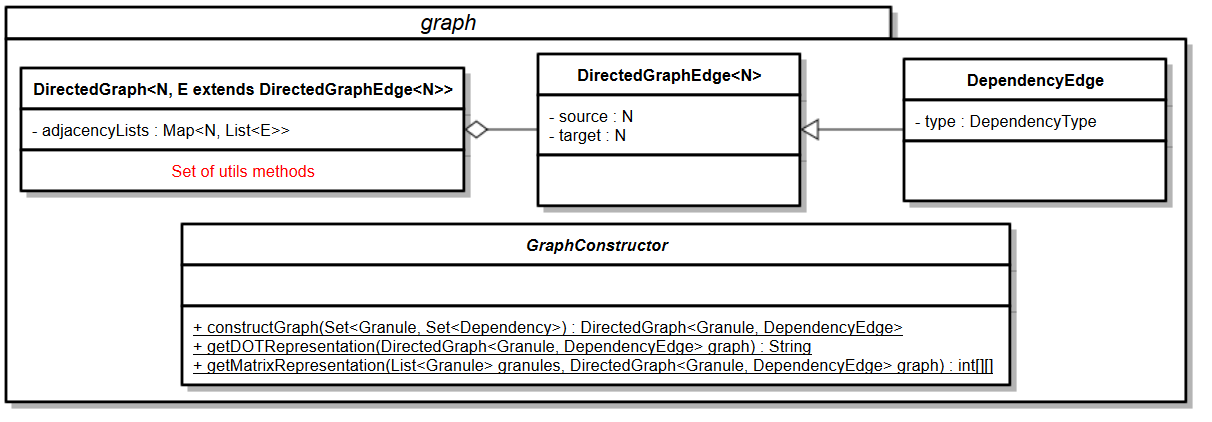
\includegraphics[width=\textwidth]{img/uml/graph.png}
        \caption{Diagramme de classes (UML) du package \texttt{graph}}
    \end{figure}

    \paragraph{}Le package \texttt{graph} a pour objectif de mettre à disposition de l’application un graphe structurant un ensemble de dépendances et offrant différents algorithmes permettant d’effectuer des calculs sur ce graphe. 
    
    \paragraph{}Ce package est composé d’une classe principale \texttt{DirectedGraph} qui définit un graphe orienté, implémenté au moyen de listes d'adjacence. Les noeuds et arêtes du graphe sont des types génériques.
    
    \paragraph{}Le service \texttt{GraphConstructor} est quant à lui chargé de construire un graphe à partir d’un ensemble de \texttt{Granule} et d’un ensemble de dépendances entre ceux-ci. Il assure également la construction de la représentation au format \emph{.dot} d'un graphe orienté et sa conversion en forme matricielle (matrice d'adjacence).
    
    \paragraph{}La classe \texttt{DirectedGraphEdge} définit la structure de données utilisée pour stocker les informations concernant les arêtes. La classe \texttt{DependencyEdge} est une extension de celle-ci contenant des informations supplémentaires relatives aux dépendances (type et multiplicité).

\subsubsection{Package metrics}

    \begin{figure}[h!]
        \centering
        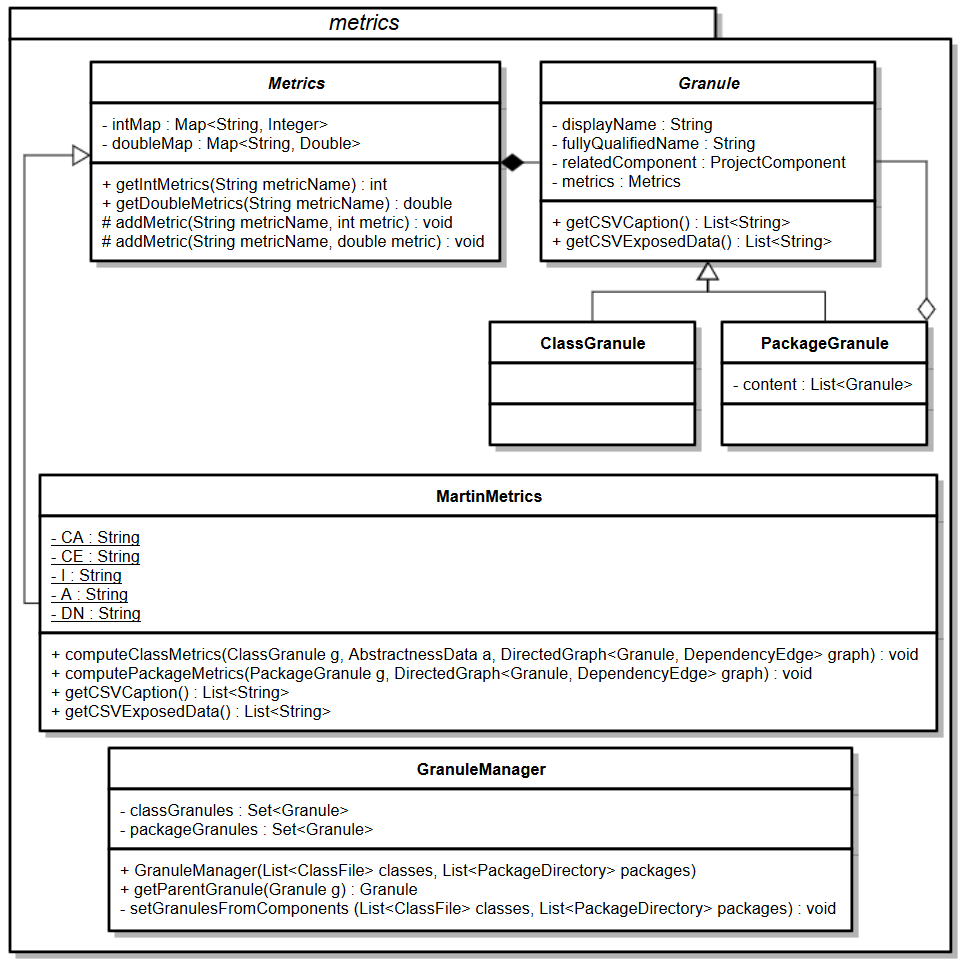
\includegraphics[width=\textwidth]{img/uml/metrics.png}
        \caption{Diagramme de classes (UML) du package \texttt{metrics}}
    \end{figure}

    \paragraph{}Le package \texttt{metrics} contient les classes permettant de réaliser le calcul de métriques selon le niveau de granularité (tels que les packages et les classes), ainsi que des classes permettant de représenter les granules.

    \paragraph{}Les classes \texttt{Granule}, \texttt{ClassGranule} et \texttt{PackageGranule} forment une instance du pattern composite générée à partir des données fournies par le package \texttt{project}. Les formes des deux structures sont très similaires, l'intérêt de passer de l'une à l'autre est de se débarrasser des références vers les fichiers de code. La conversion entre celles-ci est effectuée par l'intermédiaire du service \texttt{GranuleManager}. La structure du package \texttt{metrics} permet également de hiérarchiser les différents granules du projet (par niveau de granularité). 
    
    \paragraph{}La classe abstraite \texttt{Granule} représente ainsi les composants à analyser. Implémentant l'interface \texttt{CSVRepresentable}, elle fournit les méthodes relatives à l'exportation des résultats des métriques au format CSV. La représentation des métriques est déléguée à leur implémentation. Les classes \texttt{ClassGranule} et \texttt{PackageDirectory} représentent respectivement les classes et les packages et contiennent leurs métriques. La classe \texttt{GranuleManager} fournit des services permettant de gérer les différents granules d'un projet.
    
    \paragraph{}L'ensemble des métriques décrites par Martin\cite{Martin:1994} est implémenté par la classe \texttt{MartinMetrics} qui hérite de la classe abstraite \texttt{Metrics}. Cette dernière permet d'apporter des possibilités d'extension. Ainsi, il sera possible, pour un futur utilisateur d'ajouter ses propres métriques. Le stockage des différentes composantes des métriques est permis grâce à deux \texttt{HashMap}, dont le tuple (clé, valeur) représente le nom et la valeur de la composante. Leur différence se trouve dans le type de la valeur en question ; l'une d'entre elles prendra des \texttt{int} comme valeur alors que l'autre prendra des \texttt{double}.

\subsubsection{Package presentation}
    \begin{figure}[h!]
        \centering
        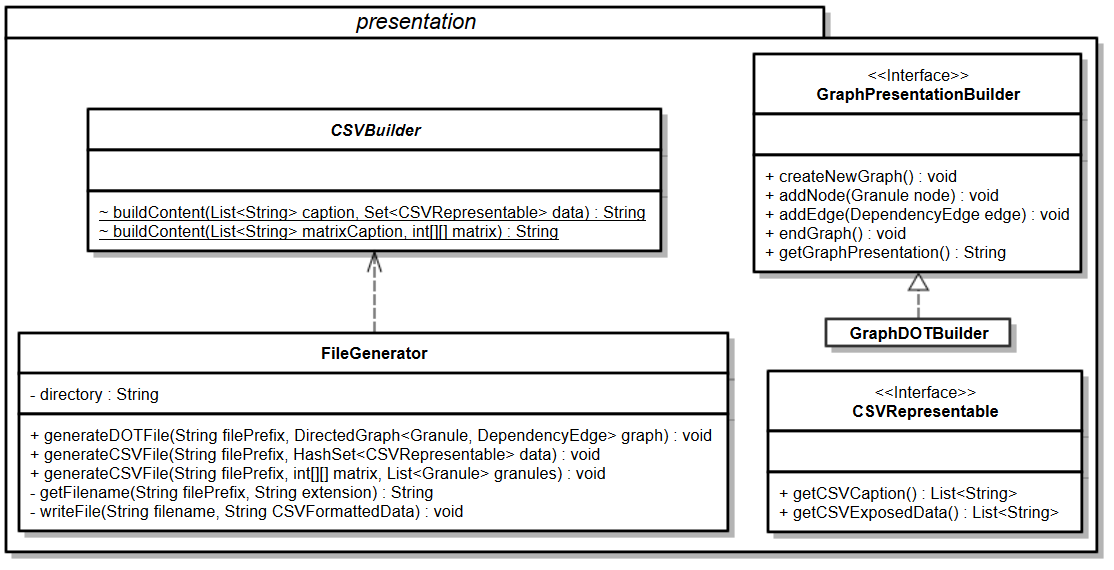
\includegraphics[width=\textwidth]{img/uml/presentation.png}
        \caption{Diagramme de classes (UML) du package \texttt{presentation}}
    \end{figure}

    \paragraph{}Le package \texttt{presentation} fournit les classes nécessaires à la génération de différents rapports d'analyse sous forme de fichiers. 
    
    \paragraph{}A cette fin, nous avons mis en place deux interfaces permettant la représentation des structures de données de l'application :
    \begin{itemize}
        \item \texttt{GraphPresentationBuilder} : Définit les méthodes de représentation d'un graphe de dépendances sous la forme d'une chaîne de caractères.
        \item \texttt{CSVRepresentable} : Définit les méthodes permettant de représenter un objet au format CSV. L'interface définit les méthodes \texttt{getCaption} qui permet de fournir la légende du fichier CSV et \texttt{getExposedData} qui permet de fournir les données de l'instance qui seront exportées. Ces deux méthodes retournent une \texttt{List} de \texttt{String}.
    \end{itemize}
    
    \paragraph{}Dans l'ensemble de notre projet, nous trouvons trois classes qui implémentent l'interface \texttt{CSVRepresentable} :
    \begin{itemize}
        \item \texttt{Granule} : Expose le nom du granule et l'ensemble des valeurs des métriques qui lui sont associées. 
        \item \texttt{Metrics} : Expose le nom des composantes de la métrique ainsi que ses valeurs. Les méthodes de l'interface \texttt{CSVRepresentable} ne sont pas directement définies dans cette classe abstraite : ce sont les classes qui en héritent qui auront pour rôle de les implémenter.
        \item \texttt{Dependency} : Expose le granule source, le granule destination, le type et la multiplicité de la dépendance.
    \end{itemize}
    
    \paragraph{}A partir d'un ensemble d'instances de \texttt{CSVRepresentable}, le service \texttt{CSVBuilder} va construire une chaîne de caractères au format CSV. 
    
    \paragraph{}Une implémentation de l'interface \texttt{GraphPresentationBuilder} est donnée dans notre projet par la classe \texttt{GraphDotBuilder} qui aura pour but de construire la représentation du graphe de dépendances au format DOT.
    
    \paragraph{}Enfin, la génération des fichiers (au format DOT et CSV) sera réalisée par l'intermédiaire de la classe \texttt{FileGenerator}.

\subsection{Choix d'implémentation}

    \subsubsection{Comparaison des méthodes d'analyse}
    \label{methodsComparison}
    \paragraph{}Il existe deux méthodes pour analyser un programme Java : l'analyse de bytecode et l'analyse de code source. Le but de cette section est de dresser une comparaison entre celles-ci.
    
    \paragraph{Informations récupérables}Tout d'abord, le code source contient des informations perdues à la compilation et qui ne peuvent donc pas être retrouvées dans le bytecode. En effet, toutes les informations liées aux types génériques sont effacées (elles ne sont utilisées que dans le but d'effectuer des vérifications à la compilation) empêchant ainsi la détection de certaines dépendances.
    
    Par exemple, si on dispose du programme suivant :
    
    \begin{minipage}{(\textwidth/2) - 0.6cm}
        \begin{lstlisting}
public class A {

}
        \end{lstlisting}
    \end{minipage}
    \hspace{0.5cm}
    \begin{minipage}{(\textwidth/2) - 0.6cm}
        \begin{lstlisting}
public class B {
    private List<A> aList;
}
        \end{lstlisting}
    \end{minipage}
    
    On remarque que B possède une liste de A (il s'agit donc d'une dépendance d'association, B ayant une agrégation de A). Lorsque l'analyse passera sur l'attribut \texttt{aList}, on s'attend à ce que son type soit \texttt{List<A>} afin de pouvoir extraire la dépendance vers A. Si on effectue l'analyse sur le code source, on obtient effectivement ce résultat. Si cependant on analyse le bytecode du même programme, le type de \texttt{aList} sera uniquement \texttt{List}, l'information de généricité du type \texttt{List} étant effacée à la compilation. En utilisant la méthode analysant le bytecode, aucune dépendance de B vers A ne sera donc détectée sur ce programme. L'analyse de code source n'a pas cette limitation car les informations de types génériques y sont écrites.
    
    Certaines autres indications sont également absentes du bytecode : la déclaration de nom de package (bien que récupérable depuis le nom complet de la classe), les déclarations \texttt{import}, ... Ceci n'est pas gênant car l'application n'exploite pas ces informations.
    
    \paragraph{Outils et facilité de mise en place} Il existe plusieurs outils / bibliothèques permettant d'exploiter ces deux méthodes :
        \bigbreak
        \begin{itemize}
            \item[\textbf{Bytecode}] Les principales bibliothèques sont les suivantes :
            \begin{itemize}
                \smallbreak
                \item[\textit{API java.lang.reflect}]L'introspection est la manière la plus rapide d'extraire des données depuis un code compilé car il s'agit d'une API directement intégrée au JDK. Le chargement des classes est facile et le parcours des attributs et méthodes l'est également. Il est cependant plus difficile de charger une classe et l'analyser via cet API si cette même classe est déjà chargée dans la JVM et que les versions diffèrent (par exemple, si on analyse l'API Java 5 en lançant le logiciel sur une JVM Java 8, beaucoup de classes déjà chargées en mémoire portent le même nom mais comportent énormément de différences). Ceci est dû au fait que pour récupérer des informations sur une classe via l'introspection, il est nécessaire de la charger dans la JVM comme s'il s'agissait d'une classe faisant partie de notre logiciel. En outre, cette API ne permet pas l'accès au corps des méthodes, empêchant par là même l'extraction de la grande majorité des dépendances de liens d'utilisation.
                \smallbreak
                \item[\textit{ASM}\footnotemark] \footnotetext{\url{https://asm.ow2.io/}}La bibliothèque permettant l'analyse (et même la modification) de bytecode la plus populaire est ASM. Cette dernière, contrairement à l'introspection, ne nécessite pas de charger les classes dans la JVM et permet l'accès aux instructions situées dans le corps des méthodes. Il s'agit cependant d'une bibliothèque externe et son utilisation nécessite d'implémenter certaines de ses interfaces (en suivant notamment le pattern \emph{Visitor}) afin d'accéder au code, ce qui rend son adoption un peu moins rapide que celle de l'introspection. Cependant, elle permet d'extraire toutes les informations contenues dans le bytecode, permettant ainsi de récupérer la plupart des dépendances.
            \end{itemize}
            \bigbreak
            \item[\textbf{Code source}] Les principales bibliothèques sont les suivantes :
            \begin{itemize}
                \smallbreak
            	\item[\textit{Eclipse JDT}]La bibliothèque JDT, faisant partie du projet Eclipse, est l'API de \emph{parsing} de code Java la plus populaire. A partir de code source Java, JDT construit un arbre de syntaxe abstrait (AST) qui peut ensuite être parcouru (en suivant le pattern \emph{Visitor}) afin d'effectuer certaines actions sur les nœuds correspondant à des instructions qui nous intéressent. Cette bibliothèque existe depuis longtemps, est très activement maintenue par bon nombre de développeurs et possède un support complet des spécifications de toutes les versions du langage Java (de 1 à 11). Elle présente cependant deux points faibles : sa difficulté à mettre en place et sa relative lenteur. En effet, afin d'utiliser des fonctionnalités avancées de JDT, il faut faire appel à plusieurs autres API du projet Eclipse. De plus, de par sa grande complexité en terme de fonctionnalités offertes, JDT prend du temps et de la mémoire pour parser un grand nombre de fichiers source et construire leur AST. Ceci est d'autant plus vrai si on veut résoudre tous les liens existant entre les symboles (par exemple entre l'instanciation d'une classe et sa déclaration).
            	
            	\smallbreak
            	\item[\textit{JavaParser}\footnotemark] \footnotetext{\url{https://javaparser.org/}}JavaParser est une autre API de \emph{parsing} de code source Java, la deuxième plus populaire après JDT. Elle est activement maintenue, supporte toutes les versions de Java de 1 à 11 et a un fonctionnement similaire à JDT : elle construit un AST à partir du code source Java et permet le parcours de celui-ci via une implémentation du pattern \emph{Visitor}. La construction des AST est plus rapide qu'avec JDT, mais JavaParser semble ne pas pouvoir résoudre tous les liens dans le code. Son utilisation est cependant plus aisée car il n'est pas nécessaire de faire appel à d'autres API pour accéder aux fonctionnalités plus avancées.
            \end{itemize}
        \end{itemize}
        

        \paragraph{Remarques annexes}Il existe quelques différences supplémentaires (bien que moins importantes que les points précédents) qui méritent d'être exposées:
        \begin{itemize}
        	\item\textbf{Complexité en temps} : Quel que soit l'outil utilisé, il est plus rapide d'effectuer une analyse de bytecode qu'une analyse de code source. Cela est dû au fait que beaucoup de liens sont résolus à la compilation et ne nécessitent pas d'être recalculés (par exemple, lors de l'instanciation d'une classe, on connaît directement son nom complet) là où les parseurs de code source doivent les construire.
        	\item\textbf{Disponibilité des fichiers} : Bien que cela survienne très rarement, il est possible que l'utilisateur veuille analyser l'architecture d'une application dont il ne possède que les fichiers de code compilé. Dans ce cas, l'analyse de code source ne peut se faire (où alors il faut décompiler le code, procédé assez délicat) et il faut impérativement utiliser l'analyse de code compilé. Dans le cas contraire (le plus courant), on ne possède que le code source. On peut alors obtenir le bytecode aisément en compilant le programme. Il est donc possible d'utiliser autant l'analyse de code source que l'analyse de bytecode.
        	\item\textbf{Informations divergentes} : Au cours de la compilation, certaines portions du programme sont transformées. Parmi ces modifications, nous avons repéré (mais il en existe potentiellement d'autres\footnote{\url{https://docs.oracle.com/javase/specs/}}) :
        	\begin{itemize}
        	    \item l'ajout de deux méthodes dans les classes d'énumération : \texttt{values} et \texttt{valueOf}.
        	    \item l'ajout d'un attribut dans les classes internes qui référence leur classe englobante.
        	    \item l'ajout d'un constructeur par défaut si celui-ci n'est pas spécifié.
        	\end{itemize}
        	Ceci implique que le code compilé possède une structure légèrement différente du code source. L'analyse de bytecode détecte donc des dépendances et méthodes que l'analyse de code source n'est pas en mesure de récupérer.
        \end{itemize}
       
    \subsubsection{Choix décisifs et limitations}
    \label{limit}
    
        \paragraph{Conservation des deux méthodes d'analyse}Bien que l'analyse de code source s'avère être la plus efficace, nous avons décidé de conserver également notre parseur de code compilé. En effet, ceci permet de mener des expériences comparatives entre ces deux méthodes, ce qui constitue un des besoins principaux du projet. Cependant, il pourrait être opportun de supprimer l'analyse de bytecode car il est compliqué de rester cohérent dans la gestion des spécificités des deux parseurs (cf. \ref{methodsComparison}).
        
        \paragraph{Performance et optimisation}L'analyse du code s'effectue en deux temps : analyse du niveau d'abstraction et analyse des dépendances. Cette séparation induit une complexité en temps plus importante car chaque fichier est parsé deux fois. De plus, l'analyse étant l'étape la plus longue, l'impact sur la durée d'exécution est non négligeable. Cependant, les performances ne constituant pas un besoin pour le client, nous avons fait le choix de privilégier une architecture plus propre en conservant la distinction entre les deux analyses. Les différents tests que nous avons effectués montrent de bonnes performances, y compris sur des projets de très grande taille (cf. \ref{tab:testPerf}).
        
        \paragraph{Gestion de la multiplicité des dépendances}Nous ne considérons qu'une seule et unique dépendance par type et par granule. Par exemple s'il y a dix dépendances d'utilisation d'un granule A vers un granule B, on n'en considère qu'une seule. Certaines interprétations de la métrique de Martin tiennent compte de la multiplicité des dépendances\cite{Martin:2003}, d'autres non\cite{Spinellis:2006}. Les deux cas semblent donner des résultats satisfaisants. Nous avons pris le parti de ne pas exploiter cette information par simplicité d'implémentation.
        
        \paragraph{Dépendances externes}Nous ne considérons les dépendances qu'au sein d'un même projet. En effet, bien qu'il soit facile de récupérer les dépendances efférentes vers des granules externes, l'inverse ne peut pas être exhaustif. Ce choix a donc pour but d'éviter d'extraire un nombre disproportionné de dépendances efférentes par rapport aux dépendances afférentes, ce qui perturberait les calculs des métriques. De ce fait les dépendances vers des bibliothèques externes, par exemple l'API standard, sont ignorées.
        
        \paragraph{Éléments ignorés}Nous avons fait le choix d'ignorer certains éléments lors des analyses, pour diverses raisons. En voici la liste :
        \begin{itemize}
            \item \textbf{Les constructeurs} : Lors du comptage du nombre de méthodes d'une classe, les constructeurs sont ignorés. Ce choix est motivé par le fait qu'à la compilation, un constructeur par défaut est ajouté aux classes n'en possédant pas. Ceci entraîne des incohérences entre les mesures effectuées sur le code source et le code compilé.
            \item \textbf{Les classes internes et anonymes} : A la demande du client et afin de simplifier l'analyse, les classes internes et anonymes sont ignorées par les deux analyses.
        \end{itemize}
        \textbf{Classes et fichiers} : L'application considère que chaque fichier contient une unique classe portant le même nom que celui-ci. De ce fait, toute autre classe est ignorée.
        
\newpage
\section{Tests}
    \paragraph{}Nous avons, tout au long de notre projet, développé une série de tests permettant de contrôler le bon fonctionnement de notre implémentation. Les outils et méthodes que nous avons utilisés ayant évolué au cours de la période de développement, ces tests nous ont permis d'identifier les problèmes de régression. Enfin, au travers de la mise en œuvre des tests directement liés à notre domaine d’étude (analyse et métrique), nous avons pu appréhender les spécificités et ainsi améliorer le cœur de notre programme.
    
    \paragraph{}Pour la mise en oeuvre de ces tests, nous avons utilisé le framework \textbf{JUnit 5}.
    
    \paragraph{}Les composants de notre application ayant été soumis à une série de tests sont les suivants : 
    \begin{itemize}
    	\item L'exploration du système de fichiers et la création d'une structure représentative du projet.
    	\item Les métriques et leurs différents calculs.
    	\item Le graphe, ses primitives ainsi que les services qui y sont associés.
    	\item L’analyse de code.
    \end{itemize}

\subsection{Infrastructure de test}

    \paragraph{Vérité terrain}Le package \texttt{analysis} ne pouvant pas être testé de manière triviale, nous avons mis en oeuvre une \textbf{vérité terrain annotée} qui nous a permis de vérifier la bonne concordance des données de dépendances et des données d’abstraction extraites par notre application avec les données réellement présentes dans un projet Java.
    
    Cette vérité terrain est constituée d’un ensemble de projets Java présentant des cas divers de dépendances et d'abstraction. Nous avons mis en place un système d’annotation Java permettant de simplifier la saisie et la création d'éléments de cette vérité terrain.
    
\begin{lstlisting}[caption={Exemple de classe annotée}]
$$@ClassInfo(
    $$numberOfMethod = 1,
    $$numberOfAbstractMethod = 0,
    $$Ca = 2,
    $$Ce = 3,
    $$I = 0.6,
    $$A = 0,
    $$Dn = 0.4
$$)
$$@Dependency(dependencyTo = A.class, type = DependencyType.Inheritance)
public class B extends A {
    $$@Dependency(dependencyTo = C.class, type = DependencyType.Aggregation)
    private C c;
    $$@Dependency(dependencyTo = D.class, type = DependencyType.UseLink)
    public void doSomething() { D d = new D(); }
}
\end{lstlisting}

    \paragraph{}Une classe \texttt{GroundTruthManager} a pour but de charger en mémoire les différents projets composant la vérité terrain et offre des méthodes d'accès à ces différentes données. Le code des tests de nos parseurs est ainsi simplifié.

\subsection{Tests unitaires et d'intégration}

    \paragraph{}Le développement de tests unitaires s'est révélé compliqué à cause de notre pipeline de traitement. En effet, certains packages de notre application ne peuvent pas fonctionner seuls et nécessitent d'être intégrés dans leur contexte de fonctionnement. Nous avons tout de même réalisé des tests qui vérifient le fonctionnement correct de notre implémentation pour chacun des packages de notre projet (excepté \texttt{presentation}).
    
    \paragraph{Package project}Obtenir une bonne représentation structurelle d'un projet est l'un des points principaux de notre implémentation. Dans cette mesure, nous testons cette fonctionnalité (présente dans le package \texttt{project}) pour les deux types d'exploration de fichiers (sources et compilés).
    
    \paragraph{Package analysis}L'analyse de code constituant le coeur de notre projet, nous testons les parseurs de couplage et de niveau d'abstraction pour les deux méthodes d'analyse (code source et bytecode). Pour ce faire, nous parcourons l'ensemble des projets de la vérité terrain en vérifiant la conformité des données des annotations avec les données extraites. 
    
    \paragraph{Package metrics}Au niveau du package \texttt{metrics}, nous avons testé en premier lieu la validation des valeurs des métriques en fournissant des données incohérentes et en vérifiant la levée d'une exception correspondante. Nous avons, dans un second temps, annoté chaque classe avec les valeurs attendues pour les métriques (annotation \texttt{ClassInfo}). Nous avons ensuite vérifié la correspondance entre ces données et celles réellement calculées par l'application.
    
    \paragraph{}La comparaison à l'échelle des packages est moins évidente. Nous avons, comme pour les classes, envisagé d'utiliser des annotations, appliquées cette fois sur le fichier \texttt{package-info}. Cependant, l'extraction de ces annotations s'est avérée plus complexe. En effet, les fichiers \texttt{package-info}, tout comme les fichiers \texttt{module-info}, ne sont pas compilés. Ceci rend la lecture des annotations impossible avec notre implémentation actuelle (lecture par introspection).
    
    \paragraph{Package graph}Nous avons également testé que la structure de graphe que nous proposons est correcte. Pour ce faire, nous avons repris les primitives essentielles qui sont utilisées dans le cadre du calcul des métriques. Nous avons également testé le service de création de graphe et sa bonne intégration dans le pipeline de notre projet.
    
\subsection{Tests de performance}

    \paragraph{}Nous avons effectué des tests de performance. Ces derniers ont consisté en l’exécution de l’application sur des projets Java plus ou moins larges (dont notamment l'API Java elle-même). Ces tests nous ont permis d’obtenir un tableau représentatif des performances de notre application.
    
    Les tests de performance ont été effectués sur la configuration suivante :
    \begin{itemize}
        \item \textbf{Java} : Oracle JRE 1.8 revision 201 (Win x64)
        \item \textbf{Système d'exploitation} : Windows 10 v. 1809
        \item \textbf{Processeur} : i7 8700K 4.7Ghz
        \item \textbf{RAM} : 16Go DDR4
    \end{itemize}
    
    \begin{center}
        \label{tab:testPerf}
        \begin{tabular}{|c|c|c|c|}\hline
            Projet & Nombre de classes & Nombre de packages & Temps d'exécution \\ \hline
            Oracle JDK 1.8 & 7651 & 486 & 10 min 29 s \\ \hline
            JUnit 5 & 435 & 58 & 0 min 15 sec \\ \hline
            JMetrics & 41 & 6 & 0 min 2 sec \\ \hline
        \end{tabular}
    \end{center}


\subsection{Tests de fonctionnement}

    \paragraph{Comparaison avec JDepend} Afin de situer notre implémentation de la métrique de Martin par rapport à une autre déjà existante (cf. \ref{existingAnalysis}), nous avons analysé plusieurs codes avec notre application et JDepend en parallèle. Il en est ressorti que les valeurs des métriques calculées par les deux programmes étaient très éloignées. Les raisons de ce problème sont diverses :
    \begin{itemize}
        \item JDepend effectue une analyse sur le bytecode (à l'aide d'un parseur écrit \textit{from scratch}). Il est plus complet que notre parseur de bytecode utilisant l'introspection mais moins que notre parseur de code source (à cause des limitations du bytecode, cf. \ref{methodsComparison}). Que ce soit avec l'une ou l'autre des méthodes de notre application, les ensembles de dépendances extraits sont alors trop différents pour être comparés.
        \item JDepend tient compte des dépendances vers des bibliothèques externes dans le calcul de \emph{Ce}, mais pas dans celui de \emph{Ca} (en effet, il est techniquement impossible de connaître tous les granules existants en dehors d'un projet qui dépendent d'un granule en particulier). Ceci induit une certaine incohérence dans les valeurs de couplage, avec un \emph{Ce} souvent très élevé par rapport au \emph{Ca}. De ce fait, la plupart des granules ont une instabilité élevée. Les granules très concrets ont alors une distance à la séquence principale très faible la plupart du temps. En outre, étant donné que les granules concrets constituent une majorité dans bon nombre de projets (il y a souvent plus d'une implémentation pour chaque abstraction), JDepend affiche une distance moyenne très faible sur tous les codes analysés.

        De notre côté, nous avons choisi d'ignorer entièrement les dépendances externes. La conséquence de cette décision est une valeur de \emph{Ce} moins élevée, entraînant une valeur d'instabilité réduite. Il en résulte une distance plus grande que celle rapportée par JDepend.
    \end{itemize}
    Pour ces raisons, nous n'avons pas jugé pertinentes les expérimentations menées avec JDepend.




\newpage
\section{Résultats \& Interprétations}

    \paragraph{Données extraites}A l'exécution de notre application, plusieurs fichiers sont générés (au format CSV et DOT) permettant d'exposer les données de l'analyse à l'utilisateur. Ces données sont les mesures de dépendances sous forme de graphe (représentation graphique ou matricielle) ou de liste, et les données de métriques. Ces données sont classées par niveau de granularité (\emph{class scale} et \emph{package scale}).

\subsection{Présentation}

    \paragraph{Représentations proposées}Afin d'offrir à l'utilisateur des outils d'interprétation des données brutes extraites par notre analyse, nous avons mis en place une série de scripts Python permettant la lecture et l'étude des fichiers CSV générés. Les différentes représentations proposées sont les suivantes (les \emph{plots} présentés exposent les données de l'analyse de notre propre programme au niveau de granularité des packages) :

    \begin{itemize}
        \item \textbf{Histogramme (Métriques)} : Cette première représentation est la plus simple. Elle nous permet d'étudier les différentes composantes de la métrique sous la forme d'histogrammes.
        \begin{figure}[h!]
            \centering
            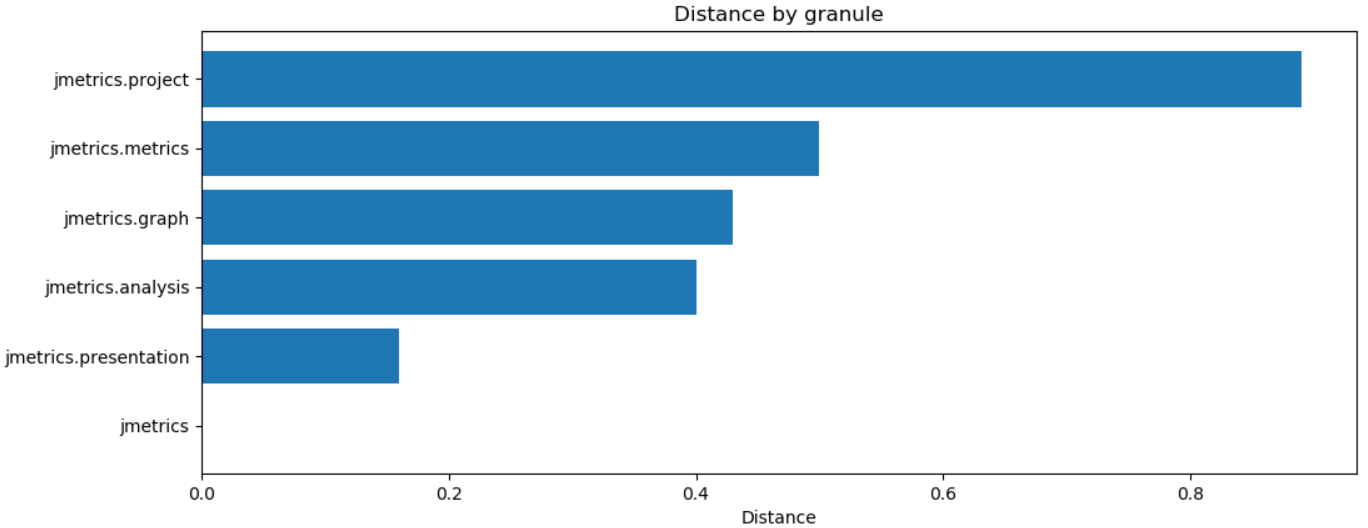
\includegraphics[width=\textwidth]{img/plot/metrics_histogram_distance.png}
            \caption{Histogramme de la composante Dn}
        \end{figure}
        
        \item \textbf{Histogramme multicolore (Dépendances)} : Cette représentation nous permet d'étudier le poids des types de dépendances dans les composantes de couplage. Ainsi, cette représentation permet une étude de l'impact des types de dépendances (et de manière indirecte, de la multiplicité) sur la valeur de stabilité. Elle étudie de manière disjointe les données de couplage afférent et efférent (un seul axe étant disponible pour l'affichage des valeurs). Nous étudions les données de couplage de manière conjointe au moyen d'une autre représentation (Représentation 2D) décrite ci-dessous.
        \begin{figure}[h!]
            \centering
            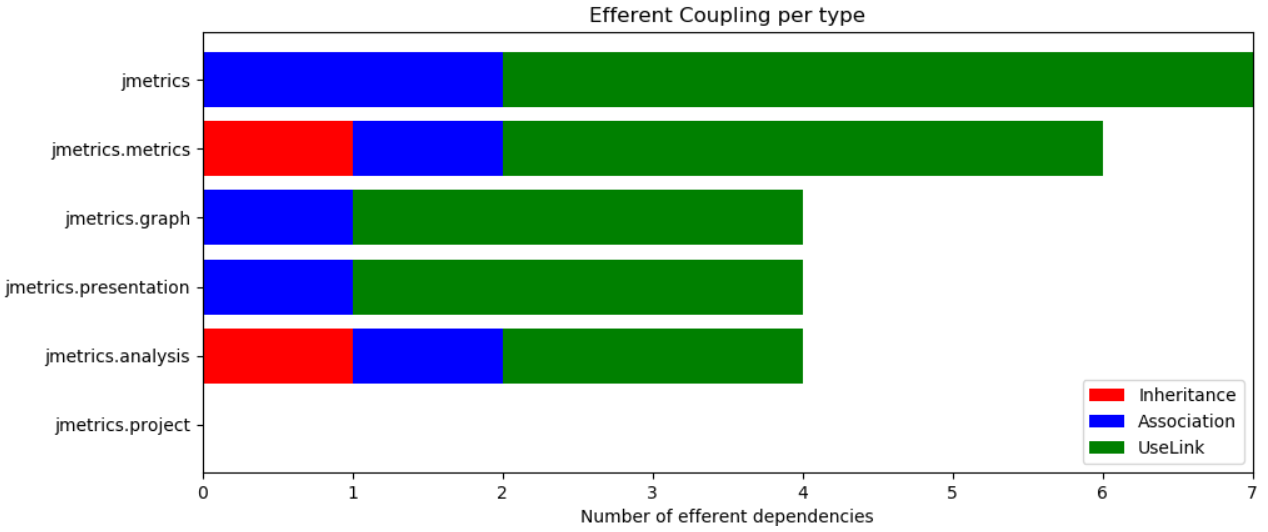
\includegraphics[width=\textwidth]{img/plot/dependencies_histogram.png}
            \caption{Histogramme du couplage efférent}
        \end{figure}
        
        \vspace{25mm}
        \item \textbf{Représentation 2D (Instabilité et Abstraction)} : Cette représentation met en relation les données d'instabilité et d'abstraction sur un axe orthogonal. Cette représentation permet d'afficher les différents granules en fonction de leur stabilité et de leur niveau d'abstraction. A l'image de ce que décrit Martin dans son article, nous positionnons sur le plan les \emph{zones de souffrance et d'inutilité} ainsi que la séquence principale (cf. \ref{fig:mainSeq}). Cette représentation graphique, bien que soumise à certaines critiques, est très représentative de la métrique énoncée par Martin.
        
        En survolant un point du plan, il est possible d'obtenir les coordonnées du point (données d'abstraction et de stabilité), sa distance à la séquence principale et la liste des granules présents sur cette position.
        \begin{figure}[h!]
            \centering
            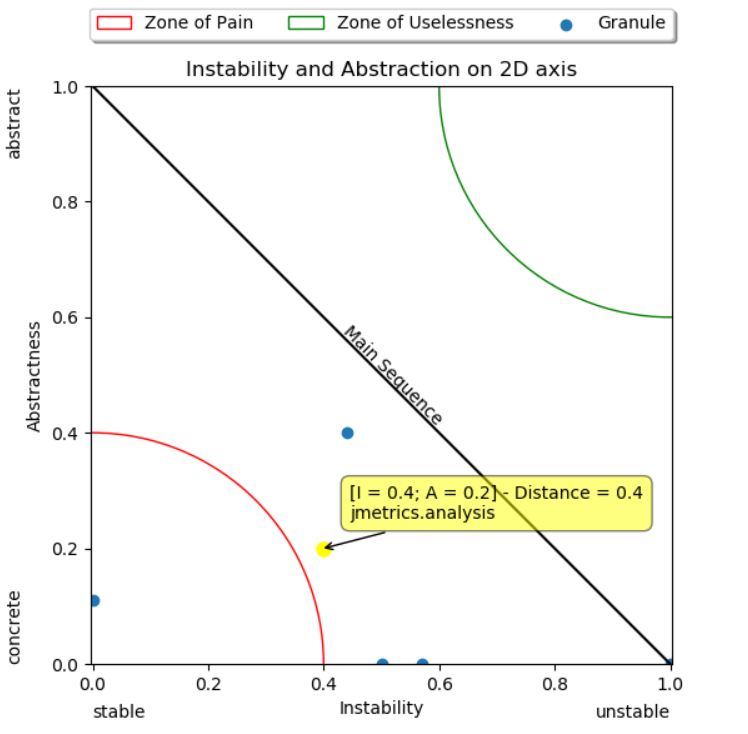
\includegraphics[scale=0.59]{img/plot/2Daxis_insta_abs.png}
            \caption{Positionnement des granules sur la Main Sequence}
        \end{figure}
        
        \item \textbf{Représentation 2D (Couplage afférent et efférent)} : Cette représentation met en relation les données de couplages afférent et efférent sur un axe orthogonal. Cette représentation nous permet d'étudier la stabilité en séparant les propriétés de responsabilité et d'indépendance. De plus, elle nous permet d'étudier les extrema des valeurs de couplage. Nous faisons ici abstraction du type des dépendances pour nous concentrer sur les valeurs de couplage uniquement.
        \begin{figure}[h!]
            \centering
            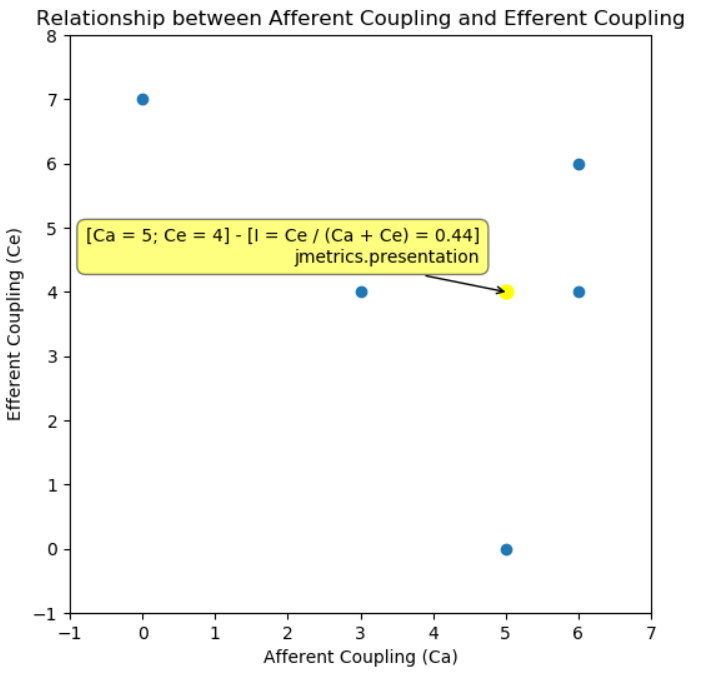
\includegraphics[scale=0.59]{img/plot/coupling2daxis.png}
            \caption{Couplage afférent et efférent sur axe orthogonal}
        \end{figure}
        
        \item \textbf{Analyse statistique des métriques} : Enfin, un dernier script a été mis en place dans le but d'étudier les valeurs statistiques usuelles appliquées aux composantes de métriques. Ce script permet d'afficher sur la sortie standard les valeurs de moyenne, médiane, variance et de écart-type à l'ensemble des composantes de la métrique.
    \end{itemize}


\newpage
\subsection{Expérimentations}

    \subsubsection{Analyse des (GoF's) Design Pattern}
    \paragraph{}Nous avons, conjointement à l'unité d'enseignement PDP, une unité d'enseignement Architecture logicielle dans laquelle nous découvrons les Design Patterns exposés par les auteurs du \emph{Gang of Four}\cite{GoF:1994}. Dans ce contexte, nous avons souhaité créer une passerelle entre ces deux unités d'enseignement en procédant à une étude de l'analyse d'implémentations de ces design patterns par notre programme.

    \paragraph{}La motivation ayant mené à l'élaboration des design patterns étant la production d'architectures flexibles, extensibles, maintenables et réutilisables, leur étude à l'aide de la métrique de Martin semble être intéressante. De plus, nous pouvons aisément trouver, sur internet, des catalogues de petits programmes mettant en oeuvre les différents patterns ce qui constitue un avantage supplémentaire. 

    \paragraph{}Nous nous intéresserons ici à des implémentations dans leur forme minimale. Considérer de telles implémentations nous permet d'obtenir une forte \textbf{reproductibilité}. En effet, dans leur version minimale, les implémentations de pattern possèdent toutes des valeurs de métriques presque similaires.

    \paragraph{}Nous noterons cependant que, découplées de tout environnement, certaines classes peuvent avoir des valeurs de métriques qui ne correspondent pas à leurs valeurs dans une utilisation normale du pattern. Par exemple, une classe \emph{Singleton}, ou encore une classe \emph{Component} (classe mère d'une instance de pattern composite) aura tendance à avoir un couplage afférent important qui n’apparaîtra pas dans les exemples. 
    
    De plus, comme indiqué par les auteurs du GoF, bien qu'il soit tout à fait possible de faire collaborer plusieurs patterns, nous ne verrons ici aucun cas d'une telle collaboration.
    
    \paragraph{Échec critique}Nous avons, dans une première tentative, effectué des mesures sur l'ensemble des implémentations minimales des patterns présentés dans le dépôt \textbf{Refactoring\_Guru}\footnote{\url{https://github.com/RefactoringGuru/design-patterns-java}} de l'auteur \emph{Alexey Pyltsyn}. Cependant, les valeurs moyennes que nous avons obtenues n'était pas suffisamment révélatrices pour être indiquées ici. Nous avons donc fait le choix d'étudier de manière plus spécifique un sous ensemble de patterns.

    \paragraph{Études de cas}Nous étudierons donc plus en détail ici l'application de la métrique de Martin aux trois patterns suivants : \textbf{Abstract Factory} (\emph{Creational}), \textbf{Composite} (\emph{Structural}) et \textbf{Command} (\emph{Behavioral}). Pour chaque pattern étudié, nous présenterons leurs participants, et pour chacun d'entre eux, leurs caractéristiques.

    \textbf{Remarque importante} : Les design patterns ne représente que des modèles théoriques qu'il faut adapter à chaque situation. Les caractéristiques exposées ci-dessous se concentrerons sur une vision générale et ne correspondront donc pas à l'ensemble des implémentations possibles.
    
    \begin{figure}[H]
        \centering
        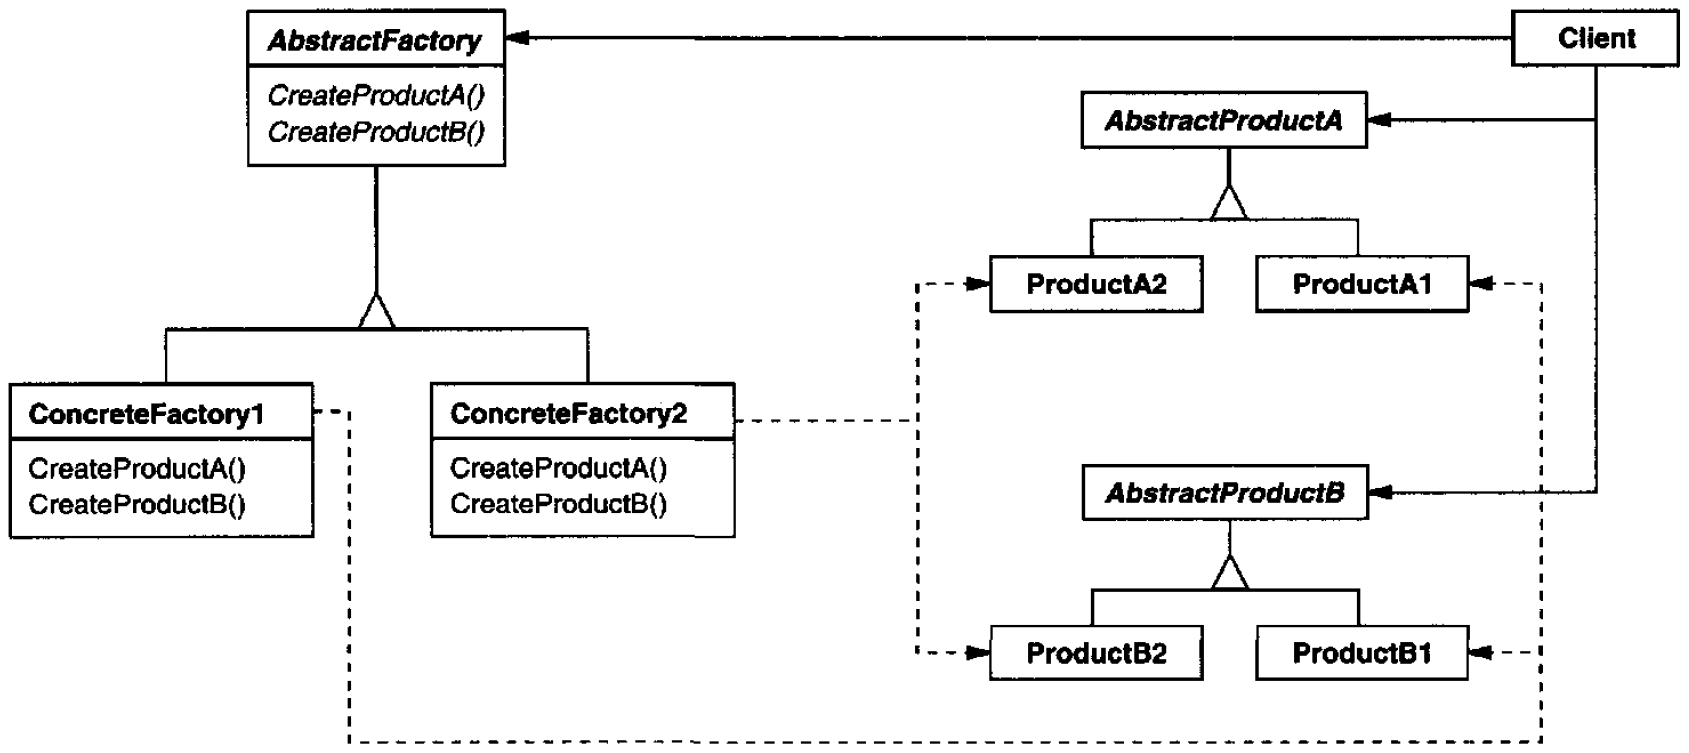
\includegraphics[scale=0.35]{img/pattern/abstract_factory.png}
        \caption{Structure du pattern \emph{Abstract Factory} définie par le GoF}
    \end{figure}
    \paragraph{Abstract Factory}Les participants du pattern sont les suivants : 
    \begin{itemize}
        \item \textbf{AbstractFactory} : La fabrique abstraite a un niveau d'abstraction élevé. Elle possède un couplage afférent lié au nombre de clients maintenant une référence vers elle, et un couplage efférent relatif au nombre de ses produits abstraits.
        \item \textbf{ConcreteFactory} : Les fabriques concrètes ont un niveau d'abstraction nul. Elles possèdent un couplage afférent nul, et un couplage efférent relatif au nombre de produits liés : elles ont donc une forte instabilité. Cela implique qu'elles ont une distance faible à la Main Sequence.
        \item \textbf{AbstractProduct} : Les produits abstraits ont un niveau d'abstraction élevé. Avec un Ca important et un Ce nul, ils ont une instabilité proche de 0. Ils se situent donc proche de la Main Sequence.
        \item \textbf{ConcreteProduct} : Les produits concrets ont un niveau d'abstraction nul et un couplage afférent et efférent faible (possiblement égale).
        \item \textbf{Client} : Enfin, le client possède une référence vers l'ensemble des classes abstraites du modèle. Ces classes étant supposées stable, les dépendances respectent le SDP.
    \end{itemize}
    
    \vspace{2mm}\hrule
    
    \begin{figure}[H]
        \centering
        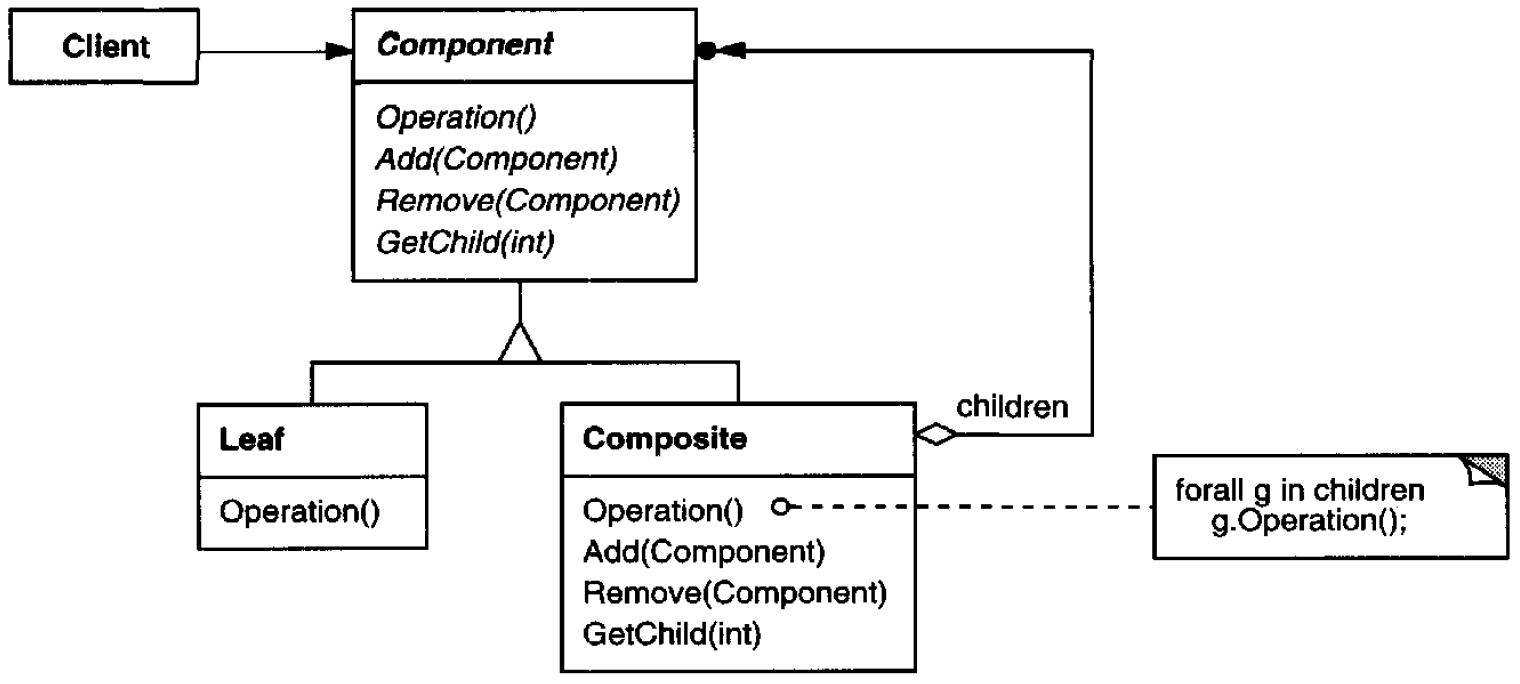
\includegraphics[scale=0.35]{img/pattern/composite.png}
        \caption{Structure du pattern \emph{Composite} définie par le GoF}
    \end{figure}
    \paragraph{Composite}Les participants du pattern sont les suivants :
    \begin{itemize}
        \item \textbf{Component} : Le composant a un niveau d'abstraction élevé. Avec un couplage efférent nul et un couplage afférent élevé, le composant à une forte stabilité. Cela implique qu'il est situé proche de la Main Sequence.
        \item \textbf{Composite} : Le composite est un élément concret. Les couplages afférent et efférent sont directement liés aux besoins de spécialisations et au rôle de la classe.
        \item \textbf{Leaf} : Même remarque que pour le Composite.
        \item \textbf{Client} : Le client maintient généralement des références vers la classe mère de la structure (le composant étant stable, cette dépendance respecte le SDP). Il pourra tout de même maintenir des références vers les classes filles dans le but procéder à des contrôles de typage ou des spécialisations.
    \end{itemize}
    
    \vspace{2mm}\hrule
    
    \begin{figure}[H]
        \centering
        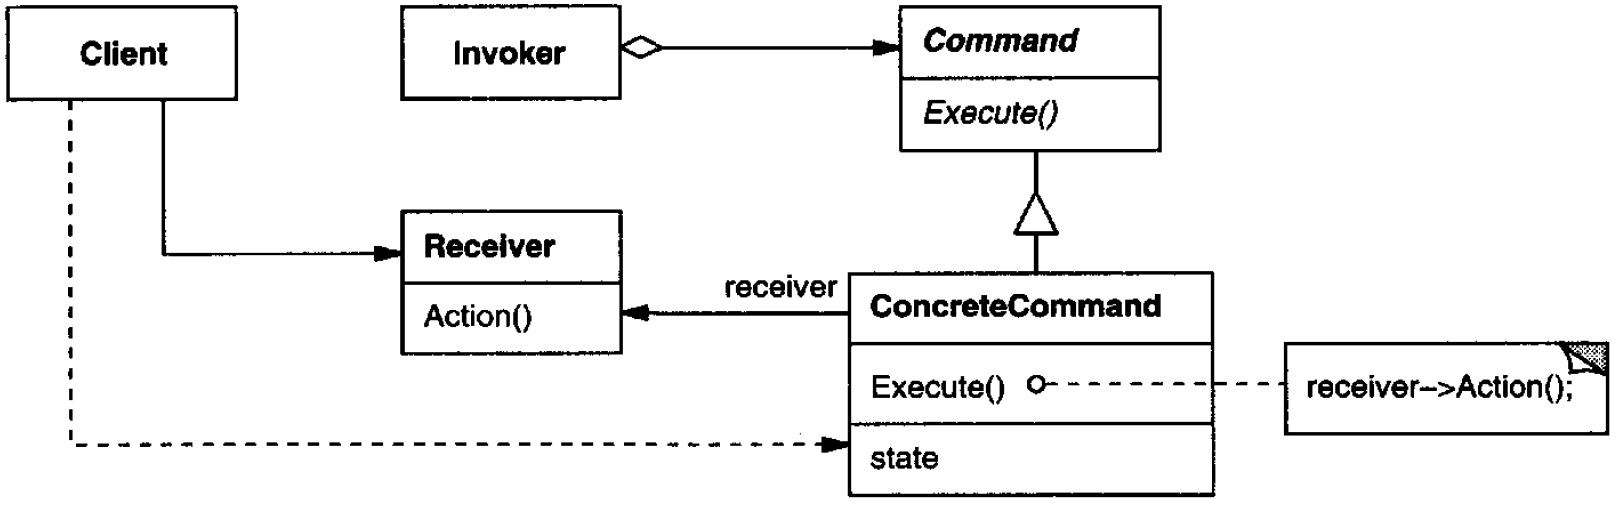
\includegraphics[scale=0.35]{img/pattern/command.png}
        \caption{Structure du pattern \emph{Command} définie par le GoF}
    \end{figure}
    \paragraph{Command}Les participants du pattern sont les suivants :
    \begin{itemize}
        \item \textbf{Command} : La classe commande est fortement abstraite. Avec un couplage afférent fort et un couplage efférent nul, la classe est d'une grande stabilité et se situe donc sur la Main Sequence.
        \item \textbf{ConcreteCommand} : Les commandes concrètes ont un niveau d'abstraction nul. Elles ont un couplage afférent faible, réduit au nombre de client capable de \emph{lancé} la commande. Leur couplage efférent est cependant possiblement élevé dès lors que leurs états maintient des références vers leurs environnement. De plus 
        \item \textbf{Invoker} : L'invocateur maintient une référence vers la liste des commandes (il y a donc un respect du SDP).
        \item \textbf{Client} : Le client maintient ici des références vers les commandes concrètes qui sont des éléments concret et possiblement instable.
    \end{itemize}
    
    \paragraph{Conclusion}Après ces différentes études de cas, nous remarquons que les principes sous-jacent à la métrique semblent être largement respectés par les design patterns. En effet, ces principes sont généralement adoptés par les développeurs de manière implicite, il est donc normal de les retrouver dans ces modèles théoriques. Nous trouvons certains cas de violation, mais la métrique ne représentant pas un absolu, il est parfois nécessaire de déroger à certaines règles.


\newpage
\section{Conclusion et perspective}
\subsection{Bilan}

    \paragraph{Travail effectué}La compréhension de la métrique, au travers des différents articles que nous avons étudié et de ses notions théoriques sous-jacentes a constitué la première étape de notre travail. Après de multiples discutions avec notre client, nous avons pu améliorer notre compréhension générale du projet et déterminer ses besoins. Par la suite, nous avons passé la plus grande partie de notre temps à concevoir notre application et à y implémenter les différentes fonctionnalités souhaitées. Enfin, nous avons tenté d'exploiter les différentes données que nous avons pu obtenir grâce à notre application en créant une série de visualisations de données. Ces différentes étapes nous ont permis d'améliorer continuellement notre compréhension du sujet, ce qui fut un préalable à la rédaction de ce mémoire.

    \paragraph{Difficultés rencontrées}La compréhension du domaine, préambule à l'élaboration du projet, a constitué une grande difficulté. En effet, des concepts tels que la stabilité sont longtemps restés peu clair. Nous avons ainsi dû retravailler ces différentes notions théoriques à de multiples reprises. 
    
    \paragraph{}Au début du projet, sans aucune expérience dans l'analyse de code, la comparaison des méthodes d'analyse fut une tâche complexe. Nous avons ainsi passé beaucoup de temps sur l'étude de ces différents outils permettant ces analyses.

    \paragraph{Conclusion}Nous avons réussi à satisfaire l'ensemble des besoins exposés par le client. Cependant, dans un soucis d'amélioration continue, nous exposons tout de même une série d'évolutions envisageables dans la section suivante.
    

\subsection{Perspectives}
    
    \paragraph{}Ce projet est, comme tout projet, améliorable. Nous avons présenté dans la partie limitation (cf. \ref{limit}) une liste de points sur lesquels nous pourrions revenir.
    
    \paragraph{}En plus de celle-ci, nous avons pensé à la mise en oeuvre de quelques améliorations :
    \begin{itemize}
    
        \item \textbf{Optimisation mémoire} : Actuellement, notre représentation des granules après analyse conserve une référence vers leur fichier/dossier. Or, d'après le pipeline, il n'est plus nécessaire d'accéder à nouveau aux fichiers après l'analyse. De ce fait, nous pourrions corriger l'implémentation afin de supprimer cette référence inutile.
        
        \item \textbf{Formats de sortie} : Les sorties de notre programme sont actuellement formatées en CSV. Ce format est pratique pour représenter une série de données partageant la même structure. En conséquence, il est nécessaire de créer un fichier par type de données à représenter (valeurs de métriques, dépendances, ...). Un format plus riche, comme le XML, pourrait permettre de représenter plus d'informations dans moins de fichiers, tout en gardant la facilité de lecture du CSV.

        \item \textbf{Visualisation de données} : En plus des différentes visualisations de données proposées, il serait intéressant de penser et de mettre en oeuvre d'autres représentations permettant une bonne interprétation des données.
        
        \item \textbf{Niveaux de granularité} : Il serait intéressant de considérer de nouveaux niveaux de granularité tels que les modules, ainsi que les attributs et méthodes au sein d'une classe.

        \item \textbf{Améliorer le calcul de métrique} : La bibliographie sur la métrique de Martin étant très vaste, il est toujours possible d'améliorer les différentes spécificités du calcul de celle-ci. 
        
        \item \textbf{Application du SDP} : Comme abordé dans la description du domaine, un calcul itératif sur le graphe permettrait de minimiser le poids des dépendances stables dans le calcul du couplage en propageant la stabilité. Il serait alors possible d'appliquer le SDP, qui n'est actuellement pas pris en compte dans la métrique.
        
        \item \textbf{Métriques supplémentaires} : Grâce à la flexibilité de notre package \texttt{metrics}, l'intégration de métriques est facilitée. On pourrait donc envisager l'ajout de métriques supplémentaires (les métriques de Chidamber et Kemerer, ...).
        
        \item \textbf{Intégration aux IDE} : Afin de faciliter l'utilisation de notre application, il pourrait être opportun de l'intégrer aux IDE les plus utilisés (Eclipse, IntelliJ, ...).
        
        \item \textbf{Gestion des releases d'un projet} : Pour voir l'évolution des métriques en fonctions des releases (fonctionnalités apportées et \emph{refactor} effectués), il pourrait être envisagé d'intégrer notre application à des outils de gestion de version (Gitlab, ...).
       
    \end{itemize}




% ----------> BIBLIOGRAPHY
\pagebreak
\bibliographystyle{alpha}
\bibliography{references}


\newpage
\begin{appendices}


\section{Analyse de projet : Exemple}

    \paragraph{}Dans le but de vérifier que l'application calcule les valeurs de métrique correctement, il est nécessaire d'écrire de petits logiciels simples présentant des configurations de dépendances différentes. Nous donnons ici un exemple élémentaire de projet ainsi que les sorties de l'application pour celui-ci.
    
\begin{minipage}{7.5cm}
\begin{lstlisting}[caption=Classe Vehicle]
public abstract class Vehicle {
    private int nbWheel;
    private ArrayList<Wheel> wheels;
    public abstract void move();
    public void setNbWheel(int i) { }
    public void addWheel(Wheel w) { }
}
\end{lstlisting}
\end{minipage}
\hspace{0.5cm}
\begin{minipage}{6cm}
\begin{lstlisting}[caption=Enumeration Material]
public enum Material {
    Plastic,
    Metal,
    Carbon
}
\end{lstlisting}
\end{minipage}
\vspace{0.5cm}
\begin{lstlisting}[caption=Classe Airplane]
public class Airplane extends Vehicle {
    @Override
    public void move() { /* ... */ }
}
\end{lstlisting}
\begin{lstlisting}[caption=Classe Car]
public class Car extends Vehicle {
    @Override
    public void move() { /* ... */ }
}
\end{lstlisting}
\begin{lstlisting}[caption=Classe Wheel]
public class Wheel {
    private Material material;
    public Material getMaterial() { return this.material; }
    public void setMaterial(Material m) { this.material = m; }
}
\end{lstlisting}



\begin{figure}[h!]
    \centering
    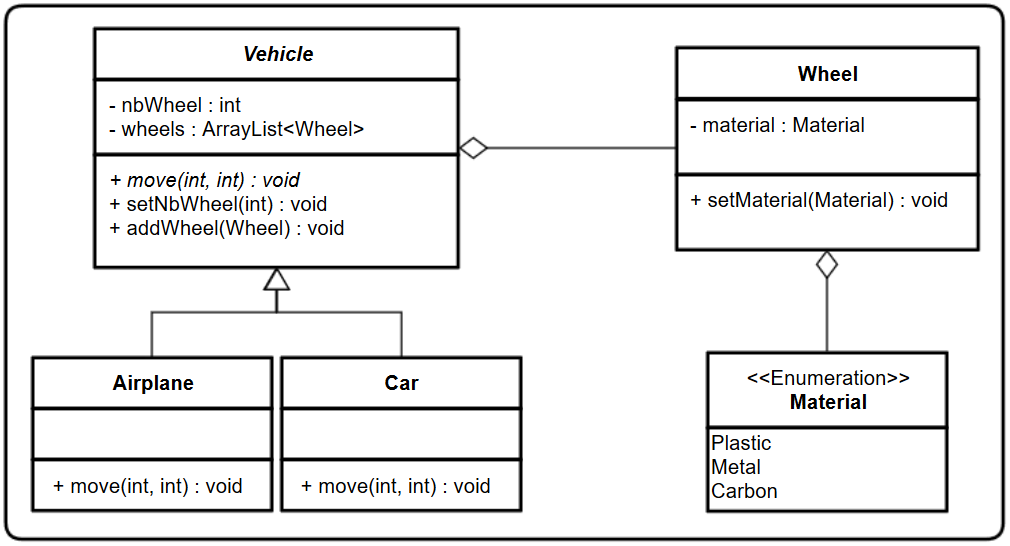
\includegraphics[scale=0.6]{img/example_uml.png}
    \caption{Diagramme de classe du projet exemple}
\end{figure}


\begin{table}[H]\caption{Tableau exposant les métriques}
    \centering
    \begin{tabular}{|c|c|c|c|c|c|}
        \hline
        \textbf{Granule} & \textbf{Ca} & \textbf{Ce} & \textbf{I} & \textbf{A} & \textbf{Dn} \\
        \hline
        \textbf{Vehicle} & 2 & 2 & 0.5 & 0.33 & 0.17 \\
        \hline
        \textbf{Material} & 2 & 0 & 0 & 0 & 1 \\
        \hline
        \textbf{Airplane} & 0 & 1 & 1 & 0 & 0  \\
        \hline
        \textbf{Car} & 0 & 1 & 1 & 0 & 0 \\
        \hline
        \textbf{Wheel} & 2 & 2 & 0.5 & 0 & 0.5 \\
        \hline
    \end{tabular}
\end{table}


\begin{figure}
    \centering
    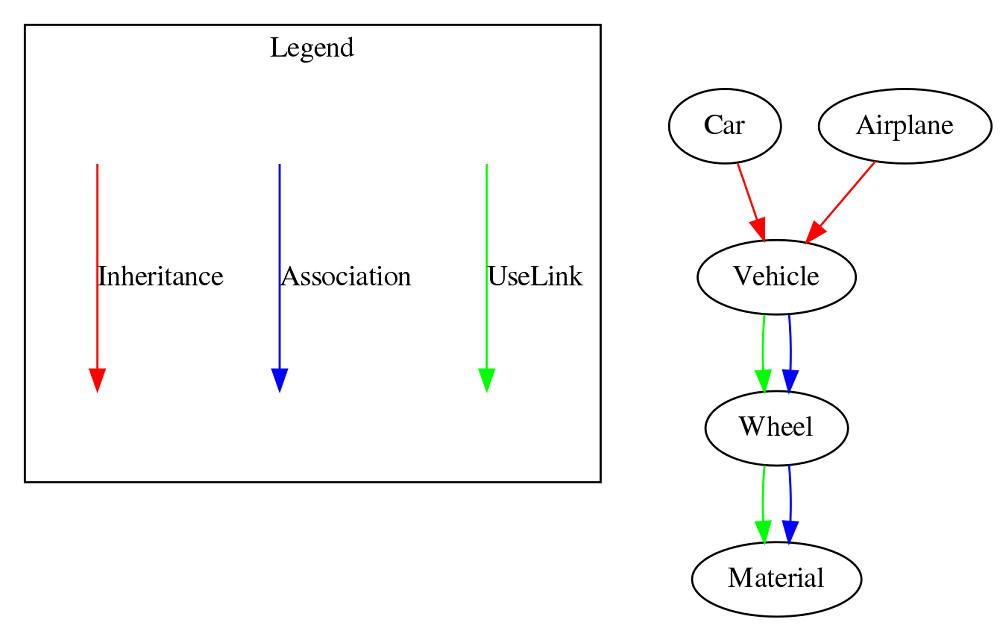
\includegraphics[scale=0.6]{img/ExampleClassesGraph.png}
    \caption{Graphe des dépendances du projet exemple construit par l'application}
\end{figure}

\end{appendices}

\end{document}
